%! Unidad 4 — El enlace químico (teoría, ejemplos resueltos, ejercicios por apartados, lectura, prácticas y situación de aprendizaje)
%! Fuente: Fuentes/Quimica/Unidad 4 (capturas 516-526 y solucionario). Texto reescrito; datos de los ejercicios cambiados y recalculados.
%! Electronegatividades: las de Pauling de la tabla tab:ud3-en (UD3): H 2,2; C 2,6; N 3,0; O 3,4; F 4,0; Cl 3,2; Br 3,0; I 2,7;
%!   S 2,6; P 2,2; Si 1,9; B 2,0; Be 1,6; Al 1,6; Li 1,0; Na 0,9; K 0,8; Mg 1,3; Ca 1,0; Ba 0,9.
%! Criterio orientativo: ΔEN ≤ 0,4 covalente apolar; 0,4-1,7 covalente polar; > 1,7 iónico.
%! Estructuras de Lewis con chemfig: \chemfig{H-\charge{90=\:,270=\:}{O}-H}. Figuras en images/UD4/ (las copiadas de
%! 2BachQuimica/FigurasSVG/UD3_Enlace_Quimico/pdf llevan otro nombre: ver progreso_temas.md).

\setchemfig{atom sep=2.2em}

\section*{Para empezar: ¿cómo trepa un gecko por el cristal?}
\addcontentsline{toc}{section}{Para empezar: ¿cómo trepa un gecko por el cristal?}

Los geckos son capaces de subir por una pared de vidrio pulido e incluso de caminar boca abajo por el techo. No usan ventosas
ni pegamento: la planta de sus dedos está cubierta de millones de pelillos microscópicos que se ramifican en puntas de unas
centésimas de micra. Cada punta se acerca tanto a la superficie que entre sus moléculas y las del vidrio aparecen unas fuerzas
eléctricas muy débiles, las \textbf{fuerzas de Van der Waals}. Una sola es insignificante, pero la suma de millones de ellas
sostiene sin problema al animal.

Son las mismas fuerzas que mantienen unidas las moléculas de agua en un vaso o que permiten licuar el nitrógeno del aire. En esta
unidad veremos por qué los átomos se unen entre sí, los distintos tipos de enlace que pueden formar y cómo el tipo de enlace
explica las propiedades de las sustancias: por qué la sal es dura pero se rompe de un golpe, por qué el cobre conduce la
corriente o por qué el agua es líquida mientras que el dióxido de carbono es un gas.

%========================================================================================
\section{Recuerda de la ESO}\label{sec:ud4-eso}
%========================================================================================

\paragraph{Energía.} La \textbf{energía} mide la capacidad de un sistema para producir cambios. En el SI se mide en
\textbf{julios} (J); también se usan la caloría (\(1~\mathrm{cal} = \qty{4.18}{\joule}\)) y el kilovatio hora
(\(\qty{1}{\kilo\watt\hour} = \qty{3.6e6}{\joule}\)). Se presenta en muchas formas (cinética, potencial, térmica, eléctrica,
química…) que se transforman unas en otras. Por convenio, la energía que \textbf{absorbe} un sistema es \textbf{positiva} y la que
\textbf{desprende}, \textbf{negativa}.

\paragraph{Ley de Coulomb.} Las cargas de distinto signo se atraen y las del mismo signo se repelen, con una fuerza
\[ F = K \, \frac{q \cdot q'}{r^2} \qquad K = \qty{9e9}{\newton\m\squared\per\coulomb\squared} \]
que es mayor cuanto mayores son las cargas y cuanto más cerca están.

\paragraph{Dipolo eléctrico.} Son dos cargas de igual valor y signo contrario, \(+q\) y \(-q\), separadas una distancia \(d\).
Se caracteriza por su \textbf{momento dipolar}, \(p = q \cdot d\).

\paragraph{Corriente eléctrica.} Es un movimiento ordenado de cargas. Para que una sustancia conduzca la corriente necesita
\textbf{cargas libres} (electrones o iones) que puedan desplazarse al aplicarle una diferencia de potencial.

\paragraph{Propiedades de los materiales.} La \textbf{dureza} es la resistencia a ser rayado (escala de Mohs, de 1 a 10); la
\textbf{tenacidad}, la resistencia a romperse al golpearlo o deformarlo, y un material poco tenaz es \textbf{frágil}; la
\textbf{conductividad} eléctrica o térmica indica lo bien que deja pasar la corriente o el calor. La mayoría de los elementos de
la tabla periódica son \textbf{metales}; los \textbf{no metales} están arriba a la derecha, y el hidrógeno, aunque se coloca en el
grupo 1, es un no metal.

\begin{exercise}
    a) Dos cargas de \qty{+2}{\micro\coulomb} y \qty{-2}{\micro\coulomb} están a \qty{3}{\cm}. Calcula la fuerza con que se atraen.
    b) ¿Cuánto vale si las separamos hasta \qty{6}{\cm}? c) ¿Qué relación tiene esto con la estabilidad de los iones de un cristal?
    \begin{solu}
        a) \(F = \dfrac{\num{9e9} \cdot \num{2e-6} \cdot \num{2e-6}}{\num{0.03}^2} = \textcolor{red}{\qty{40}{\newton}}\).
        b) Al doblar la distancia, la fuerza se divide entre 4: \textcolor{red}{\qty{10}{\newton}}. c) \textcolor{red}{Cuanto mayores
        son las cargas de los iones y más pequeños son (más cerca quedan), más se atraen} y más estable es el cristal.
    \end{solu}
\end{exercise}

%========================================================================================
\section{Estabilidad de átomos e iones}\label{sec:ud4-estabilidad}
%========================================================================================

Salvo los gases nobles, los elementos casi nunca se encuentran en la naturaleza como átomos sueltos, sino \textbf{enlazados}: el
oxígeno del aire forma moléculas \ch{O2}; el agua, moléculas \ch{H2O}, y la sal común es un cristal formado por iones \ch{Na+} y
\ch{Cl-}. ¿Por qué ocurre?

\subsection{Energía y enlace químico}

La razón es una tendencia general de la naturaleza: \textbf{un sistema es más estable cuanto menor es su energía}. Cuando dos
átomos se unen, la energía del conjunto disminuye y el sistema queda más estable que con los átomos separados.

Al acercar dos átomos aparecen fuerzas de \textbf{atracción} entre el núcleo de cada uno y los electrones del otro, y la energía
baja. Pero si se acercan demasiado, dominan las \textbf{repulsiones} entre los dos núcleos y entre las dos nubes electrónicas, y la
energía sube muy deprisa. Hay una distancia en la que la energía es \textbf{mínima}: es la \textbf{distancia de enlace}, \(d_0\),
y en ella se sitúan los átomos enlazados (figura~\ref{fig:ud4-curva}).

\begin{figure}[H]
    \centering
    \begin{tikzpicture}
        \begin{axis}[grafica, width=0.62\linewidth, height=6cm,
            xmin=40, xmax=300, ymin=-500, ymax=420,
            xlabel={Distancia entre núcleos, \(d\) (pm)}, ylabel={Energía (\unit{\kilo\joule\per\mol})},
            axis lines=middle, x label style={at={(axis description cs:0.5,-0.06)}, anchor=north},
            y label style={at={(axis description cs:-0.1,0.5)}, rotate=90, anchor=south},
            xtick={74,100,150,200,250,300}, ytick={-436,-200,0,200,400}]
            \addplot[very thick, ocre, domain=45:300] {436*((1-exp(-0.0195*(x-74)))^2-1)};
            \draw[dashed, gray] (axis cs:74,-436) -- (axis cs:74,0);
            \draw[dashed, gray] (axis cs:40,-436) -- (axis cs:74,-436);
            \node[font=\scriptsize, anchor=west] at (axis cs:112,-440) {mínimo de energía: enlace H--H};
            \node[font=\scriptsize, anchor=west, align=left] at (axis cs:105,300) {dominan las\\ repulsiones};
            \node[font=\scriptsize, anchor=south] at (axis cs:230,20) {átomos separados};
            \node[font=\scriptsize, anchor=west] at (axis cs:165,-290) {dominan las atracciones};
        \end{axis}
    \end{tikzpicture}
    \caption{Energía de dos átomos de hidrógeno según la distancia entre sus núcleos. El mínimo (\(d_0 = \qty{74}{\pico\m}\),
    \(E = \qty{-436}{\kilo\joule\per\mol}\)) corresponde a la molécula \ch{H2}.}
    \label{fig:ud4-curva}
\end{figure}

\begin{definition}[Enlace químico]
    Es el conjunto de \textbf{fuerzas} que mantienen unidos a los átomos o a los iones cuando forman moléculas o cristales.

    Al formarse un enlace se \textbf{desprende} energía. La energía que hay que \textbf{aportar} para romperlo, la \textbf{energía
    de enlace} o \textbf{de disociación}, es igual en valor a la que se desprendió al formarse.
\end{definition}

Por ejemplo, al unirse dos átomos de hidrógeno se desprenden \qty{436}{\kilo\joule} por cada mol de \ch{H2} formado, y para
separar de nuevo los átomos de un mol de \ch{H2} hay que aportar \qty{436}{\kilo\joule}. No todos los acercamientos acaban en
enlace: si la curva no tiene mínimo (como ocurre con dos átomos de helio), los átomos se separan solos, lo que explica que no
todas las combinaciones de elementos sean posibles.

\subsection{La regla del octeto}

En 1916, \textbf{W. Kossel} y \textbf{G.\,N. Lewis} se fijaron, de forma independiente, en que los gases nobles, con la capa de
valencia completa (\conf{ns^2\,np^6}), son los elementos más estables, y propusieron una teoría sencilla del enlace:

\begin{definition}[Teoría de Lewis y Kossel]
    Propusieron que:
    \begin{itemize}
        \item En el enlace solo intervienen los electrones de la \textbf{capa de valencia} (la más externa).
        \item \textbf{Regla del octeto}: los átomos \textbf{ganan}, \textbf{pierden} o \textbf{comparten} electrones hasta tener la
        configuración electrónica de un gas noble, con \textbf{ocho electrones} en su última capa (\conf{ns^2\,np^6}). Los
        elementos cercanos al helio (H, Li, Be) tienden a tener solo dos, como él (\conf{1s^2}).
    \end{itemize}
\end{definition}

La regla tiene muchas excepciones, pero funciona muy bien con los elementos representativos de los primeros periodos.

\paragraph{Diagramas de Lewis.} La \textbf{representación de Lewis} de un átomo es su símbolo rodeado de sus electrones de
valencia, dibujados como puntos (o aspas). Hasta cuatro electrones se dibujan de uno en uno, y a partir del quinto se van
emparejando (figura~\ref{fig:ud4-lewis-atomos}). El número de electrones de valencia de un elemento representativo coincide con la
última cifra de su grupo: 1 en el grupo 1, 2 en el 2, 3 en el 13, 4 en el 14… hasta 8 en el 18. Estos diagramas no dicen nada
sobre la forma en que los electrones se distribuyen en el espacio.

\begin{figure}[H]
    \centering
    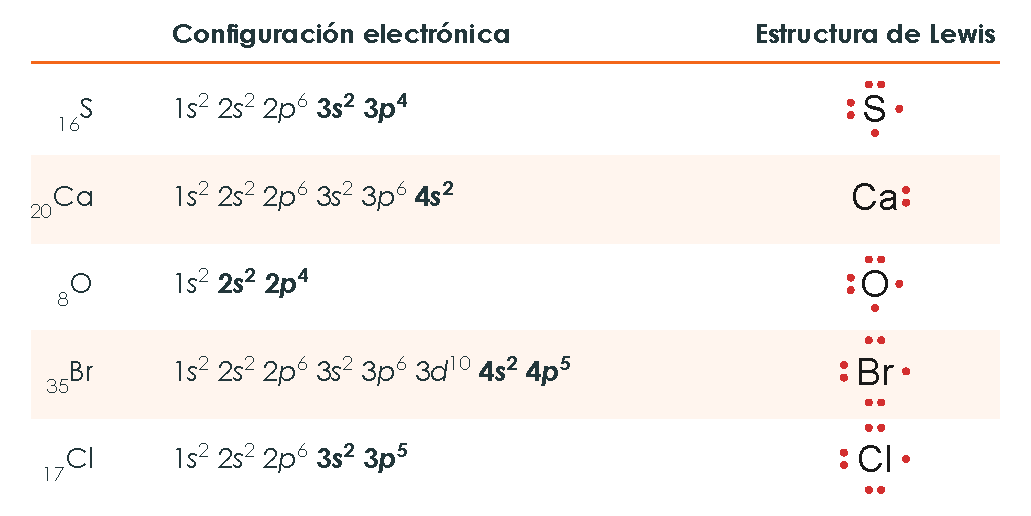
\includegraphics[width=0.62\textwidth]{images/UD4/lewis_atomos}
    \caption{Configuración electrónica y diagrama de Lewis de algunos átomos: solo se dibujan los electrones de la capa de valencia.}
    \label{fig:ud4-lewis-atomos}
\end{figure}

\paragraph{El ion más probable.} Con la regla del octeto podemos predecir qué ion formará un elemento: perderá o ganará los
electrones necesarios para quedar con la configuración del gas noble más cercano. Los metales, con pocos electrones de valencia,
los \textbf{pierden} y forman \textbf{cationes}; los no metales, con cinco, seis o siete, \textbf{ganan} los que les faltan y
forman \textbf{aniones}.

\begin{example}
    \textbf{Predecir iones.} ¿Qué ion tenderán a formar el magnesio (\(Z = 12\)) y el nitrógeno (\(Z = 7\))?

    \textbf{Solución.} Mg: \conf{1s^2\,2s^2\,2p^6\,3s^2}. Tiene 2 electrones de valencia: le es mucho más fácil perderlos que ganar
    seis, y queda con la configuración del neón: \(\ch{Mg} \rightarrow \ch{Mg^2+} + 2\,e^-\).

    N: \conf{1s^2\,2s^2\,2p^3}. Tiene 5 electrones de valencia y le faltan 3 para el octeto: tiende a ganarlos y formar el ion
    \ch{N^3-} (nitruro), también con la configuración del neón: \(\ch{N} + 3\,e^- \rightarrow \ch{N^3-}\).
\end{example}

\begin{remark}
    \textbf{Más allá del octeto.} Algunos elementos, sobre todo los de transición, no llegan a la configuración de gas noble,
    pero alcanzan una estabilidad especial con \textbf{subniveles llenos} (\conf{(n-1)d^{10}\,ns^2}, como el \ch{Zn^2+} con
    \conf{3d^{10}}) o \textbf{semillenos} (\conf{(n-1)d^5}, como el \ch{Fe^3+} o el \ch{Mn^2+}). Por eso el hierro forma
    \ch{Fe^2+} y \ch{Fe^3+}.
\end{remark}

\subsection{Tipos de enlace}

Los átomos pueden conseguir la configuración de gas noble de tres maneras: \textbf{cediendo}, \textbf{captando} o
\textbf{compartiendo} electrones. Según el tipo de elementos que se unen, hay tres tipos de enlace, y el tipo de enlace determina
las \textbf{propiedades} de la sustancia: puntos de fusión y ebullición, dureza, solubilidad, conductividad, brillo…

\begin{table}[H]
    \centering
    \caption{Los tres tipos de enlace químico}
    \vspace{-5pt}
    \begin{tabular}{@{}L{2cm}L{3cm}L{4.2cm}L{4.2cm}@{}}
        \toprule
        \textbf{Enlace} & \textbf{Entre} & \textbf{Qué ocurre} & \textbf{Qué se forma} \\
        \midrule
        Iónico & Metal y no metal & El metal cede electrones al no metal: se forman iones que se atraen & Una red cristalina de
        cationes y aniones (\ch{NaCl}) \\[3pt]
        Metálico & Átomos de un metal & Los átomos ceden sus electrones de valencia a una nube común & Una red de cationes
        rodeada de electrones (\ch{Cu}, \ch{Fe}) \\[3pt]
        Covalente & No metales & Los átomos comparten pares de electrones & Moléculas (\ch{H2O}, \ch{CO2}) o redes de átomos,
        los cristales covalentes (diamante, \ch{SiO2}) \\
        \bottomrule
    \end{tabular}
    \label{tab:ud4-tipos}
\end{table}

\begin{exercise}
    Predice el ion más probable que formarán el calcio, el fósforo, el potasio y el selenio. Escribe la configuración electrónica
    de cada átomo y de su ion.
    \begin{solu}
        Ca: \conf{[Ar]\,4s^2} \(\rightarrow\) \textcolor{red}{\ch{Ca^2+}}: \conf{[Ar]}. P: \conf{[Ne]\,3s^2\,3p^3} \(\rightarrow\)
        \textcolor{red}{\ch{P^3-}}: \conf{[Ne]\,3s^2\,3p^6} = \conf{[Ar]}. K: \conf{[Ar]\,4s^1} \(\rightarrow\)
        \textcolor{red}{\ch{K+}}: \conf{[Ar]}. Se: \conf{[Ar]\,3d^{10}\,4s^2\,4p^4} \(\rightarrow\) \textcolor{red}{\ch{Se^2-}}:
        \conf{[Ar]\,3d^{10}\,4s^2\,4p^6} = \conf{[Kr]}.
    \end{solu}
\end{exercise}

\begin{exercise}
    Con la tabla~\ref{tab:ud4-tipos}, predice qué tipo de enlace hay en: \ch{SO2}, \ch{Al}, \ch{CaBr2}, \ch{Ne} y \ch{H2S}.
    \begin{solu}
        \ch{SO2}: \textcolor{red}{covalente} (dos no metales). \ch{Al}: \textcolor{red}{metálico}. \ch{CaBr2}:
        \textcolor{red}{iónico} (metal y no metal). \ch{Ne}: \textcolor{red}{ninguno}: es un gas noble y existe como átomos sueltos.
        \ch{H2S}: \textcolor{red}{covalente}.
    \end{solu}
\end{exercise}

\begin{exercise}
    ¿Por qué el hidrógeno, el litio y el berilio no cumplen la regla del octeto? ¿Qué regla siguen?
    \begin{solu}
        \textcolor{red}{Su capa de valencia es la primera o la segunda y el gas noble más cercano es el helio}, que solo tiene dos
        electrones (\conf{1s^2}). Siguen la \textcolor{red}{«regla del dúo»}: el H gana o comparte un electrón (\ch{H-}, \ch{H2}) y
        el Li y el Be pierden 1 y 2 electrones (\ch{Li+}, \ch{Be^2+}).
    \end{solu}
\end{exercise}

\begin{exercise}
    Dibuja el diagrama de Lewis de los átomos de boro, carbono, nitrógeno, azufre y yodo.
    \begin{solu}
        Electrones de valencia: B 3, C 4, N 5, S 6 y I 7:
        \textcolor{red}{\chemfig{\charge{0=\.,90=\.,180=\.}{B}} \quad \chemfig{\charge{0=\.,90=\.,180=\.,270=\.}{C}} \quad
        \chemfig{\charge{0=\.,90=\:,180=\.,270=\.}{N}} \quad \chemfig{\charge{0=\.,90=\:,180=\.,270=\:}{S}} \quad
        \chemfig{\charge{0=\.,90=\:,180=\:,270=\:}{I}}}.
    \end{solu}
\end{exercise}

%========================================================================================
\section{Enlace iónico}\label{sec:ud4-ionico}
%========================================================================================

Cuando se encuentran un \textbf{metal} y un \textbf{no metal}, el metal, con pocos electrones de valencia y energía de ionización
baja, los \textbf{pierde} y se convierte en un \textbf{catión}; el no metal, muy electronegativo, los \textbf{gana} y se convierte
en un \textbf{anión}. Los iones, de carga opuesta, se atraen.

\begin{definition}[Enlace iónico]
    Es la unión que resulta de la \textbf{atracción eléctrica} entre \textbf{cationes} y \textbf{aniones}, formados por
    \textbf{transferencia de electrones} de los átomos de un metal a los de un no metal.
\end{definition}

Fíjate en el cloruro de sodio. El sodio (\conf{1s^2\,2s^2\,2p^6\,3s^1}) pierde su único electrón de valencia y queda como
\ch{Na+}, con la configuración del neón. El cloro (\conf{1s^2\,2s^2\,2p^6\,3s^2\,3p^5}) capta ese electrón y queda como \ch{Cl-},
con la del argón:
\[ \ch{Na} \rightarrow \ch{Na+} + e^- \qquad\qquad \ch{Cl} + e^- \rightarrow \ch{Cl-} \]
La figura~\ref{fig:ud4-lewis-iones} muestra el mismo proceso para el fluoruro de sodio con diagramas de Lewis.

\begin{figure}[H]
    \centering
    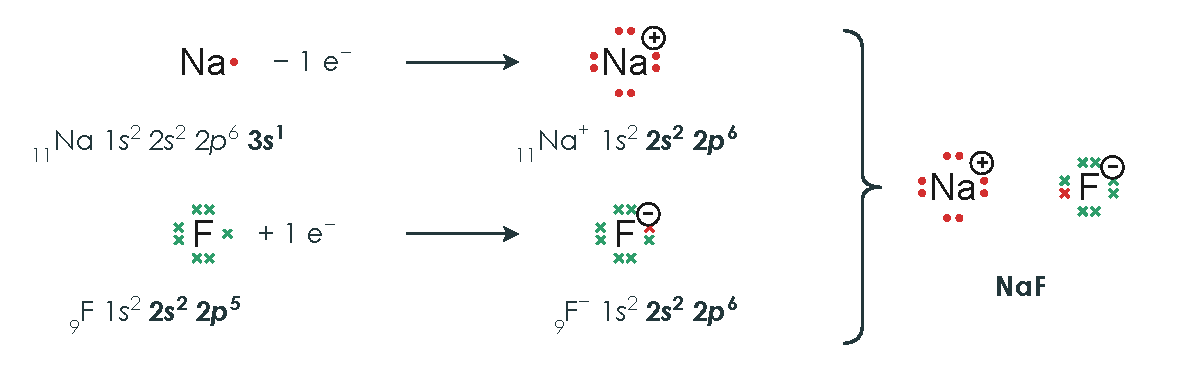
\includegraphics[width=0.62\textwidth]{images/UD4/lewis_iones}
    \caption{Formación del fluoruro de sodio: el sodio cede su electrón de valencia al flúor.}
    \label{fig:ud4-lewis-iones}
\end{figure}

\paragraph{Fórmula de un compuesto iónico.} El compuesto tiene que ser \textbf{neutro}: tiene que haber tantas cargas positivas
como negativas. La fórmula indica la \textbf{proporción} en que están los iones:
\begin{itemize}
    \item En el \ch{NaCl} hay un \ch{Na+} por cada \ch{Cl-}.
    \item En el \ch{CaF2}, dos \ch{F-} por cada \ch{Ca^2+}.
    \item En el \ch{Al2O3}, dos \ch{Al^3+} (6 cargas positivas) por cada tres \ch{O^2-} (6 cargas negativas).
\end{itemize}

\begin{remark}
    \textbf{No hay moléculas de \ch{NaCl}.} La fórmula de un compuesto iónico es una \textbf{fórmula empírica}: solo indica la
    proporción de iones en el cristal. Por eso no se habla de masa molecular, sino de \textbf{masa fórmula}: la del \ch{NaCl} es
    \(\num{23.0} + \num{35.5} = \qty{58.5}{\uma}\), y su masa molar, \qty{58.5}{\gram\per\mol}.
\end{remark}

\subsection{Redes iónicas}

Los iones no se unen por parejas: cada ion atrae a \textbf{todos} los iones de signo contrario que tiene alrededor, y se rodea del
mayor número posible de ellos. Así se forma una estructura gigante, ordenada y que se repite en las tres direcciones del espacio:
una \textbf{red cristalina} o \textbf{cristal}.

En la red, los iones se colocan de la forma más \textbf{compacta} posible, con la máxima distancia entre los iones del mismo signo y
la mínima entre los de signo contrario. El número de iones de signo contrario que rodean a cada ion es el \textbf{índice de
coordinación}, y depende de la proporción entre cationes y aniones y de su \textbf{tamaño} (figura~\ref{fig:ud4-redes}).

\begin{figure}[H]
    \centering
    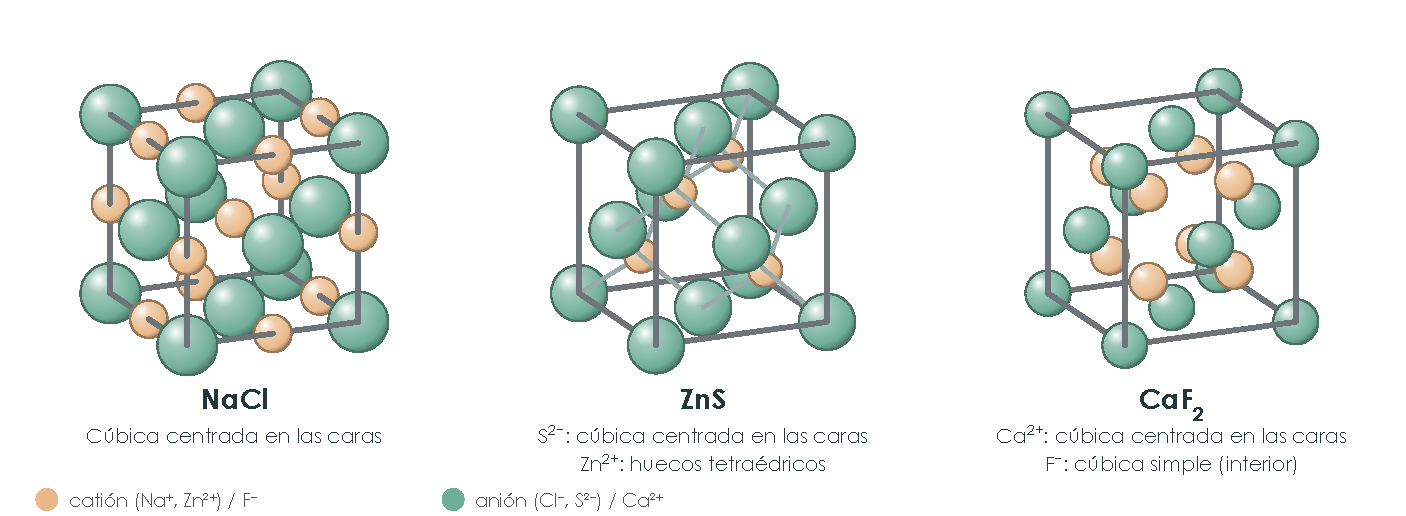
\includegraphics[width=0.85\textwidth]{images/UD4/redes_ionicas}
    \caption{Tres redes iónicas. En el \ch{NaCl} cada ion está rodeado por 6 de signo contrario; en la fluorita (\ch{CaF2}),
    cada \ch{Ca^2+} por 8 \ch{F-} y cada \ch{F-} por 4 \ch{Ca^2+}. En el \ch{CsCl} (no dibujado), el índice es 8 para los dos iones.}
    \label{fig:ud4-redes}
\end{figure}

\subsection{La energía reticular}

La formación de un cristal iónico a partir de sus elementos se puede imaginar como una serie de pasos, unos que absorben energía y
otros que la desprenden. Para el cloruro de sodio, partiendo de sodio sólido y cloro gaseoso
(tabla~\ref{tab:ud4-born-haber} y figura~\ref{fig:ud4-born-haber}):

\begin{table}[H]
    \centering
    \caption{Etapas de la formación del cloruro de sodio (ciclo de Born-Haber)}
    \vspace{-5pt}
    \begin{tabular}{@{}clL{5.2cm}r@{}}
        \toprule
        & \textbf{Etapa} & \textbf{Proceso} & \textbf{Energía (\unit{\kilo\joule\per\mol})} \\
        \midrule
        1 & Sublimar el sodio & \(\ch{Na(s)} \rightarrow \ch{Na(g)}\) & \(+108\) \\[3pt]
        2 & Disociar el cloro & \(\tfrac{1}{2}\,\ch{Cl2(g)} \rightarrow \ch{Cl(g)}\) & \(+121\) \\[3pt]
        3 & Ionizar el sodio & \(\ch{Na(g)} \rightarrow \ch{Na^+(g)} + e^-\) & \(+496\) \\[3pt]
        4 & El cloro capta un electrón & \(\ch{Cl(g)} + e^- \rightarrow \ch{Cl^-(g)}\) & \(-349\) \\[3pt]
        5 & Formar la red cristalina & \(\ch{Na^+(g)} + \ch{Cl^-(g)} \rightarrow \ch{NaCl(s)}\) & \(-787\) \\
        \midrule
        & \textbf{Proceso global} & \(\ch{Na(s)} + \tfrac{1}{2}\,\ch{Cl2(g)} \rightarrow \ch{NaCl(s)}\) & \(\mathbf{-411}\) \\
        \bottomrule
    \end{tabular}
    \label{tab:ud4-born-haber}
\end{table}

\begin{figure}[H]
    \centering
    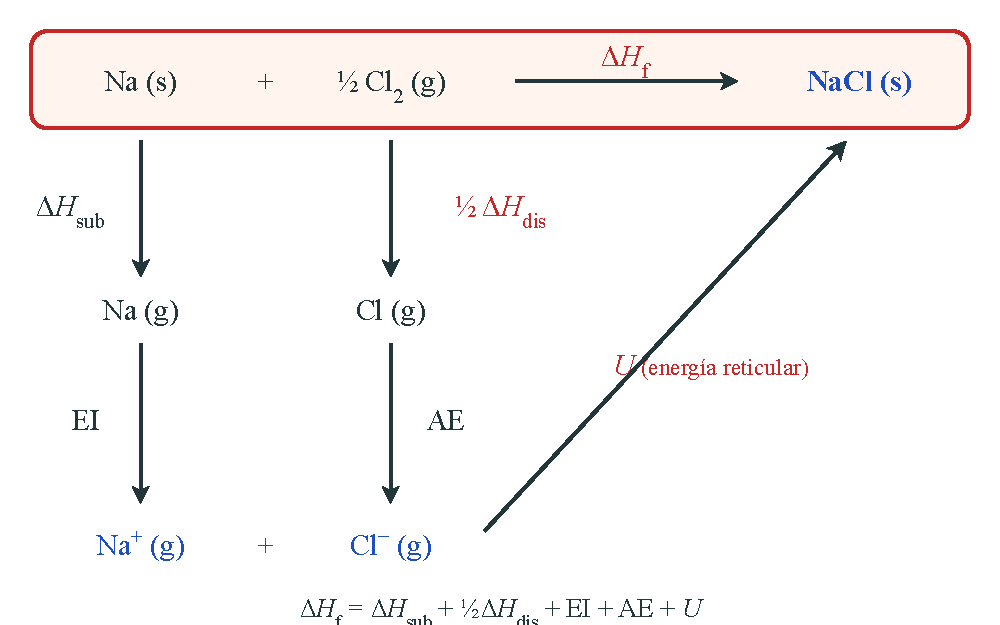
\includegraphics[width=0.62\textwidth]{images/UD4/born_haber}
    \caption{Ciclo de Born-Haber del cloruro de sodio: el camino directo (arriba) y el camino por etapas desprenden la misma
    energía. EI es la energía de ionización; AE, la afinidad electrónica, y \(U\), la energía reticular.}
    \label{fig:ud4-born-haber}
\end{figure}

Las tres primeras etapas \textbf{absorben} energía, y la cuarta desprende algo menos que lo que costó ionizar el sodio: si todo
acabara ahí, formar iones sueltos no saldría a cuenta. Lo que hace que el proceso global desprenda energía es la última etapa: la
unión de los iones gaseosos para formar el cristal.

\begin{definition}[Energía reticular]
    Es la energía que se \textbf{desprende} al formarse un mol de cristal iónico a partir de sus iones en estado gaseoso. Cuanto
    mayor es (en valor absoluto), más estable es el cristal. Es mayor cuanto \textbf{mayor} es la \textbf{carga} de los iones y
    cuanto \textbf{menor} es su \textbf{tamaño}, como predice la ley de Coulomb.
\end{definition}

\begin{example}
    \textbf{¿Cuál tiene mayor energía reticular?} Ordena de mayor a menor energía reticular (en valor absoluto) el \ch{NaCl}, el
    \ch{KCl} y el \ch{MgO}.

    \textbf{Solución.} El \ch{MgO} está formado por iones de carga \(+2\) y \(-2\), pequeños: la atracción entre ellos es unas
    cuatro veces mayor que entre iones de carga \(\pm 1\). Entre el \ch{NaCl} y el \ch{KCl}, el anión es el mismo y el \ch{Na+} es
    más pequeño que el \ch{K+} (tiene una capa menos), así que los iones quedan más cerca:
    \(\ch{MgO} > \ch{NaCl} > \ch{KCl}\). Los valores reales son \num{3850}, 787 y \qty{717}{\kilo\joule\per\mol}. Por eso el
    \ch{MgO} funde a \qty{2852}{\degreeCelsius} y el \ch{NaCl} a \qty{801}{\degreeCelsius}.
\end{example}

\begin{example}
    \textbf{Ciclo de Born-Haber del bromuro de potasio.} Calcula la energía que se desprende al formarse un mol de \ch{KBr(s)} a
    partir de sus elementos con estos datos (en \unit{\kilo\joule\per\mol}): sublimación del K, \(+89\); vaporización y disociación
    de medio mol de \ch{Br2(l)}, \(+112\); ionización del K, \(+419\); afinidad electrónica del Br, \(-325\); energía reticular del
    \ch{KBr}, \(-689\).

    \textbf{Solución.} La energía del proceso global es la suma de la de todas las etapas, porque la energía no depende del camino:
    \[ E = 89 + 112 + 419 - 325 - 689 = \qty{-394}{\kilo\joule\per\mol} \]
    Se desprenden \qty{394}{\kilo\joule} por mol de \ch{KBr} formado.
\end{example}

\subsection{Propiedades de los compuestos iónicos}

Las propiedades de los compuestos iónicos se deben a las fuerzas eléctricas, muy intensas, entre iones de distinto signo, que se
reflejan en el alto valor de su energía reticular:
\begin{itemize}
    \item Son \textbf{sólidos} a temperatura ambiente y tienen \textbf{puntos de fusión y ebullición altos}: para fundirlos hay que
    vencer la atracción entre los iones de toda la red.
    \item Son \textbf{duros}: para rayarlos hay que romper muchas atracciones entre los iones de la superficie.
    \item Son \textbf{frágiles}: al golpearlos, una capa de iones se desplaza sobre otra y quedan enfrentados iones del mismo
    signo, que se repelen y parten el cristal (figura~\ref{fig:ud4-deformacion}).
    \item Muchos son \textbf{solubles en agua} (y en otros disolventes polares): las moléculas de agua, que son dipolos, rodean a los
    iones de la superficie y los arrancan del cristal (figura~\ref{fig:ud4-disolucion}). Son insolubles en disolventes apolares.
    \item \textbf{No conducen la electricidad en estado sólido}, porque los iones no se pueden mover, pero \textbf{sí la conducen
    fundidos o disueltos}, cuando los iones quedan libres.
\end{itemize}

\begin{figure}[H]
    \centering
    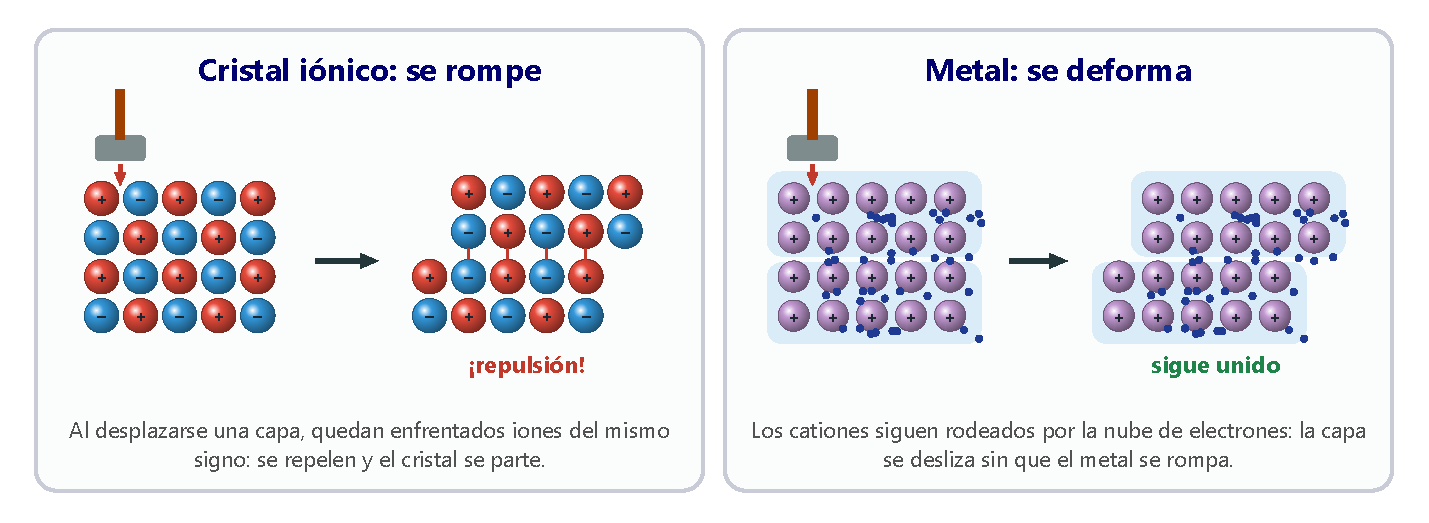
\includegraphics[width=0.85\textwidth]{images/UD4/deformacion}
    \caption{Un golpe rompe un cristal iónico, pero solo deforma un metal.}
    \label{fig:ud4-deformacion}
\end{figure}

\begin{figure}[H]
    \centering
    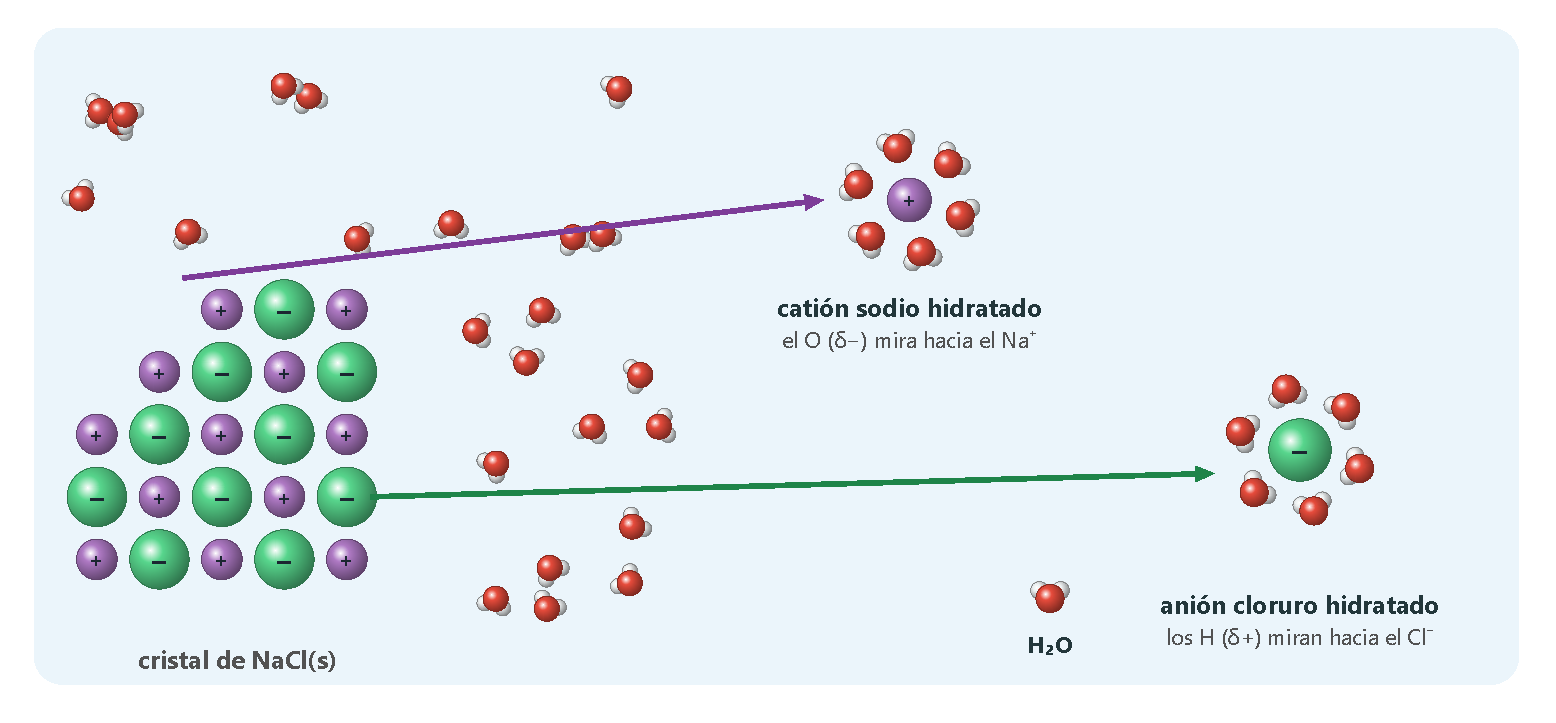
\includegraphics[width=0.8\textwidth]{images/UD2/disolucion_nacl}
    \caption{Disolución de un cristal iónico en agua: los iones quedan rodeados de moléculas de agua (iones hidratados).}
    \label{fig:ud4-disolucion}
\end{figure}

\begin{example}
    \textbf{Cómo se forma el yoduro de potasio.} Explica la formación del enlace en el \ch{KI}.

    \textbf{Solución.} El potasio es un metal y el yodo un no metal: el enlace es iónico. El K pierde su electrón 4s y el I lo
    gana, y los dos quedan con configuración de gas noble:
    \[ \ch{K}: \conf{[Ar]\,4s^1} \xrightarrow{\;-1\,e^-\;} \ch{K+}: \conf{[Ar]} \qquad\qquad
    \ch{I}: \conf{[Kr]\,4d^{10}\,5s^2\,5p^5} \xrightarrow{\;+1\,e^-\;} \ch{I-}: \conf{[Kr]\,4d^{10}\,5s^2\,5p^6} = \conf{[Xe]} \]
    Los iones \ch{K+} y \ch{I-} se atraen y se ordenan en una red cristalina en la que hay un \ch{K+} por cada \ch{I-}: \ch{KI}.
\end{example}

\begin{exercise}
    Explica cómo se forma el enlace en estos compuestos y justifica su fórmula: a) \ch{MgBr2}; b) \ch{Na2S}; c) \ch{CaO}.
    \begin{solu}
        a) \ch{Mg} \(\rightarrow\) \ch{Mg^2+} \(+\, 2\,e^-\); cada Br capta un electrón: \(\ch{Br} + e^- \rightarrow \ch{Br-}\).
        \textcolor{red}{Hacen falta dos \ch{Br-} por cada \ch{Mg^2+}}. b) Cada Na pierde un electrón y el S gana dos:
        \textcolor{red}{dos \ch{Na+} por cada \ch{S^2-}}. c) El Ca pierde dos electrones y el O gana dos:
        \textcolor{red}{un \ch{Ca^2+} por cada \ch{O^2-}}. En los tres casos los iones quedan con configuración de gas noble y
        se atraen formando una red cristalina.
    \end{solu}
\end{exercise}

\begin{exercise}
    Calcula la masa fórmula del \ch{CaCl2} y del \ch{Al2O3} (masas atómicas: Ca 40,1; Cl 35,5; Al 27,0; O 16,0). ¿Por qué no
    hablamos de masa molecular?
    \begin{solu}
        \ch{CaCl2}: \(\num{40.1} + 2 \cdot \num{35.5} = \textcolor{red}{\qty{111.1}{\uma}}\). \ch{Al2O3}:
        \(2 \cdot \num{27.0} + 3 \cdot \num{16.0} = \textcolor{red}{\qty{102.0}{\uma}}\). \textcolor{red}{Porque los compuestos
        iónicos no forman moléculas}: son redes de iones y su fórmula solo indica la proporción entre ellos.
    \end{solu}
\end{exercise}

\begin{exercise}
    Calcula la energía reticular del fluoruro de litio sabiendo que en su formación a partir de sus elementos se desprenden
    \qty{616}{\kilo\joule\per\mol} y que (en \unit{\kilo\joule\per\mol}): sublimación del Li, \(+159\); disociación de medio mol de
    \ch{F2}, \(+79\); ionización del Li, \(+520\); afinidad electrónica del F, \(-328\).
    \begin{solu}
        \(-616 = 159 + 79 + 520 - 328 + U \;\Rightarrow\; U = -616 - 430 = \textcolor{red}{\qty{-1046}{\kilo\joule\per\mol}}\).
        Es mucho mayor que la del \ch{NaCl}, porque el \ch{Li+} y el \ch{F-} son iones muy pequeños.
    \end{solu}
\end{exercise}

\begin{exercise}
    Ordena de mayor a menor punto de fusión: \ch{NaF}, \ch{NaBr}, \ch{CaO} y \ch{NaCl}. Justifica la respuesta.
    \begin{solu}
        El punto de fusión crece con la energía reticular, que aumenta con la carga de los iones y al disminuir su tamaño.
        El \ch{CaO} tiene iones de carga \(\pm 2\); los otros tres tienen el mismo catión y aniones cada vez mayores
        (\(\ch{F-} < \ch{Cl-} < \ch{Br-}\)): \textcolor{red}{\(\ch{CaO} > \ch{NaF} > \ch{NaCl} > \ch{NaBr}\)} (2613, 993, 801 y
        \qty{747}{\degreeCelsius}).
    \end{solu}
\end{exercise}

\begin{exercise}
    Al cocinar, solemos manejar un salero de vidrio. Si se nos cae al suelo, la sal no se dobla ni se aplasta: los granos se
    rompen en trocitos con caras planas. ¿Por qué? ¿Y por qué no conviene manejar aparatos eléctricos con las manos mojadas, si el
    agua pura apenas conduce la corriente?
    \begin{solu}
        \textcolor{red}{Los cristales iónicos son frágiles}: el golpe desplaza capas de iones, quedan enfrentados iones del mismo
        signo y el cristal se rompe por esos planos, que son planos. \textcolor{red}{El agua del grifo y el sudor llevan sales
        disueltas}: sus iones, libres para moverse, la hacen conductora.
    \end{solu}
\end{exercise}

%========================================================================================
\section{Enlace metálico}\label{sec:ud4-metalico}
%========================================================================================

Un trozo de cobre o de hierro, por pequeño que sea, contiene una cantidad enorme de átomos iguales. ¿Qué los mantiene unidos? Los
metales son densos, lo que indica que sus átomos están muy apretados, y conducen muy bien la electricidad, lo que exige que haya
cargas que se puedan mover. El modelo de la \textbf{nube electrónica} (o del \textbf{mar de electrones}) explica las dos cosas a
partir de dos características de los metales:
\begin{itemize}
    \item Tienen \textbf{energías de ionización bajas}: cuesta poco arrancarles electrones.
    \item Tienen \textbf{pocos electrones} de valencia (uno, dos o tres).
\end{itemize}

Según este modelo, cada átomo del metal cede sus electrones de valencia y se convierte en un \textbf{catión}. Los electrones
liberados no pertenecen a ningún átomo concreto: forman un \textbf{colectivo deslocalizado}, una nube que rodea a todos los
cationes y se mueve libremente entre ellos. Los cationes se ordenan en una \textbf{red cristalina compacta}
(figura~\ref{fig:ud4-nube}).

\begin{figure}[H]
    \centering
    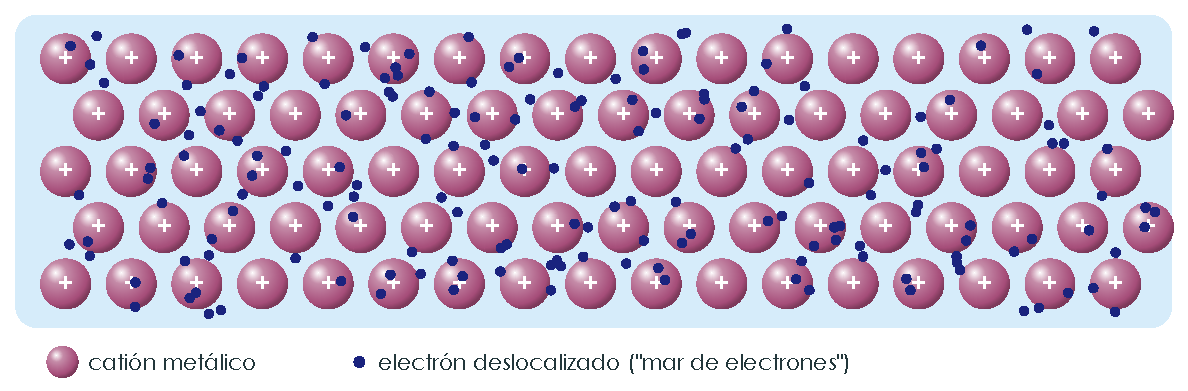
\includegraphics[width=0.6\textwidth]{images/UD4/nube_electronica}
    \caption{Modelo de la nube electrónica: cationes ordenados en una red, rodeados de electrones deslocalizados.}
    \label{fig:ud4-nube}
\end{figure}

\begin{definition}[Enlace metálico]
    Es la unión que resulta de la \textbf{atracción eléctrica} entre los \textbf{cationes} de la red y la \textbf{nube de
    electrones} deslocalizados que los rodea.
\end{definition}

\begin{example}
    \textbf{Electrones que aporta cada metal.} ¿Cuántos electrones cede a la nube electrónica un átomo de sodio y uno de aluminio?

    \textbf{Solución.} Cada metal cede los electrones de su capa de valencia:
    \[ \ch{Na}: \conf{[Ne]\,3s^1} \xrightarrow{\;-1\,e^-\;} \ch{Na+}: \conf{[Ne]} \qquad\qquad
    \ch{Al}: \conf{[Ne]\,3s^2\,3p^1} \xrightarrow{\;-3\,e^-\;} \ch{Al^3+}: \conf{[Ne]} \]
    El sodio cede \textbf{un} electrón y el aluminio, \textbf{tres}. Con más electrones en la nube y cationes de mayor carga, el
    enlace metálico del aluminio es más fuerte: funde a \qty{660}{\degreeCelsius}, frente a los \qty{98}{\degreeCelsius} del sodio.
\end{example}

\subsection{Propiedades de los metales}

\begin{itemize}
    \item Salvo el mercurio, que funde a \qty{-39}{\degreeCelsius}, son \textbf{sólidos} a temperatura ambiente. Sus puntos de
    fusión son muy variados: desde los \qty{29}{\degreeCelsius} del galio, que se funde en la mano, hasta los
    \qty{3422}{\degreeCelsius} del wolframio.
    \item Tienen \textbf{densidad alta}, porque la red de cationes es muy compacta.
    \item Son \textbf{dúctiles} (se estiran en hilos) y \textbf{maleables} (se extienden en láminas): cuando una capa de cationes
    se desliza sobre otra, la nube electrónica se adapta y sigue uniéndolos, sin que aparezcan repulsiones
    (figura~\ref{fig:ud4-deformacion}).
    \item Son \textbf{buenos conductores de la electricidad y del calor}, gracias a la movilidad de los electrones de la nube.
    \item Tienen un \textbf{brillo} característico: los electrones libres absorben la luz y la vuelven a emitir.
    \item Son \textbf{insolubles} en agua y en los disolventes habituales (algunos, como los alcalinos, reaccionan con el agua, que
    no es lo mismo). Fundidos se mezclan entre sí y forman \textbf{aleaciones}, como el bronce (cobre y estaño) o el latón (cobre y
    cinc). El acero es hierro con un poco de carbono.
\end{itemize}

\begin{remark}
    \textbf{Conductores, semiconductores y aislantes.} Un modelo más completo, la \textbf{teoría de bandas}, explica la conducción
    con los niveles de energía de los electrones del cristal (figura~\ref{fig:ud4-bandas}). En un conductor, la banda que ocupan
    los electrones de valencia se solapa con una banda vacía (de conducción) a la que los electrones pasan sin esfuerzo. En un
    aislante, entre ambas hay un gran salto de energía. En un \textbf{semiconductor}, como el silicio, el salto es pequeño: con un
    poco de energía (calor o luz) algunos electrones lo superan y el material conduce, y con ellos se fabrican los chips y las
    placas solares.
\end{remark}

\begin{figure}[H]
    \centering
    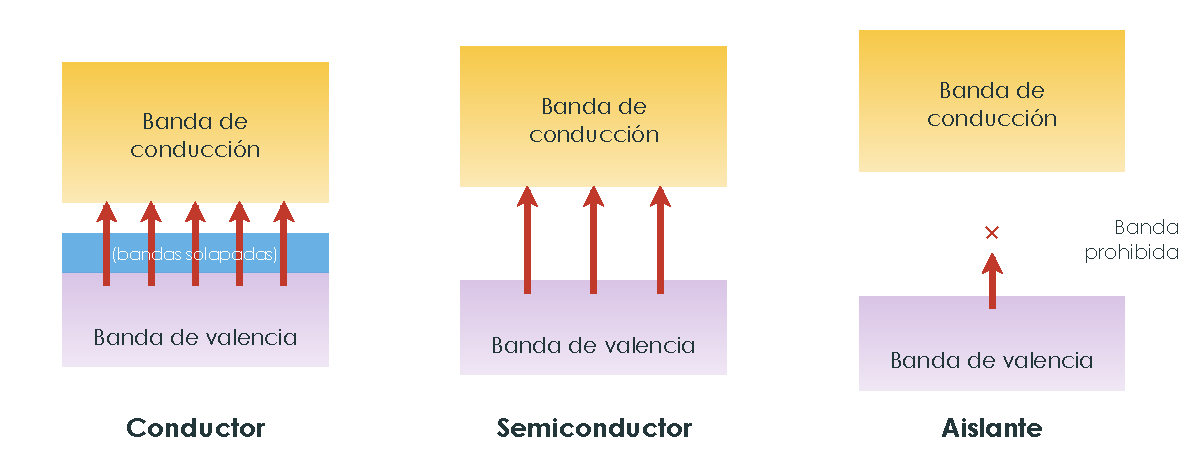
\includegraphics[width=0.65\textwidth]{images/UD4/bandas}
    \caption{Teoría de bandas: conductores, semiconductores y aislantes.}
    \label{fig:ud4-bandas}
\end{figure}

\begin{exercise}
    ¿Cuántos electrones cede a la nube electrónica un átomo de cada uno de estos metales? a) Li; b) Ca; c) Ga; d) Ba.
    \begin{solu}
        Cada uno cede sus electrones de valencia: a) Li, \conf{[He]\,2s^1}: \textcolor{red}{1}. b) Ca, \conf{[Ar]\,4s^2}:
        \textcolor{red}{2}. c) Ga, \conf{[Ar]\,3d^{10}\,4s^2\,4p^1}: \textcolor{red}{3}. d) Ba, \conf{[Xe]\,6s^2}: \textcolor{red}{2}.
    \end{solu}
\end{exercise}

\begin{exercise}
    ¿Por qué podemos hacer cables de cobre o papel de aluminio, pero no podemos hacer hilos de sal común?
    \begin{solu}
        \textcolor{red}{Los metales son dúctiles y maleables}: al deformarlos, las capas de cationes se deslizan sin que la nube de
        electrones deje de unirlas. \textcolor{red}{La sal es frágil}: al deformarla, quedan enfrentados iones del mismo signo, que
        se repelen, y el cristal se rompe.
    \end{solu}
\end{exercise}

\begin{exercise}
    Las sartenes son de metal, pero sus mangos suelen ser de plástico o de madera. ¿Por qué?
    \begin{solu}
        \textcolor{red}{Los metales conducen muy bien el calor}, gracias a los electrones libres, y el mango se calentaría tanto
        como el fondo. \textcolor{red}{El plástico y la madera son malos conductores} (sus electrones están localizados en enlaces
        covalentes) y no queman.
    \end{solu}
\end{exercise}

\begin{exercise}
    El potasio funde a \qty{63}{\degreeCelsius} y el calcio, a \qty{842}{\degreeCelsius}. Explica la diferencia con el modelo de
    la nube electrónica.
    \begin{solu}
        \textcolor{red}{El K cede un electrón y queda como \ch{K+}; el Ca cede dos y queda como \ch{Ca^2+}}, más pequeño y con más
        carga. En el calcio la nube tiene el doble de electrones y la atracción entre la nube y los cationes es mucho mayor: hace
        falta más energía para romper la red.
    \end{solu}
\end{exercise}

%========================================================================================
\section{Enlace covalente}\label{sec:ud4-covalente}
%========================================================================================

Imagina que en clase de Lengua os mandan leer dos libros y en tu casa tenéis uno y en la de un amigo, el otro. Lo más sencillo es
que os los prestéis: cada uno usa los dos libros sin comprar ninguno. Algo parecido hacen los átomos de los no metales: todos
necesitan \textbf{ganar} electrones para completar su capa de valencia, y como ninguno quiere cederlos, los \textbf{comparten}.

Fíjate en el hidrógeno. Cada átomo de H tiene un electrón; si los dos átomos juntan sus electrones en un \textbf{par
compartido}, cada uno «tiene» dos electrones y alcanza la configuración del helio:
\[ \mathrm{H}\!\cdot \;+\; \cdot\mathrm{H} \;\longrightarrow\; \mathrm{H}\!:\!\mathrm{H} \quad \text{o bien} \quad \mathrm{H{-}H} \]
Del mismo modo, cada átomo de flúor, con siete electrones de valencia, comparte uno con el otro y los dos completan el octeto
(figura~\ref{fig:ud4-F2}).

\begin{figure}[H]
    \centering
    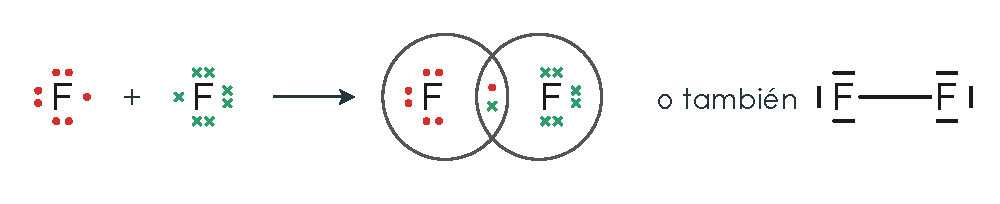
\includegraphics[width=0.55\textwidth]{images/UD4/lewis_F2}
    \caption{Formación de la molécula de flúor: el par compartido cuenta para el octeto de los dos átomos.}
    \label{fig:ud4-F2}
\end{figure}

\begin{definition}[Enlace covalente]
    Es la unión entre átomos que \textbf{comparten} uno o más \textbf{pares de electrones}, atraídos a la vez por los dos núcleos.
    Se da entre átomos de \textbf{no metales}.

    La \textbf{valencia covalente} (o covalencia) de un átomo es el número de enlaces covalentes que forma, y suele coincidir con el
    número de electrones que le faltan para completar el octeto (o con el de sus electrones desapareados).
\end{definition}

En una estructura de Lewis, cada \textbf{par compartido} o \textbf{par enlazante} se dibuja como un guion, y los pares que no se
comparten (\textbf{pares no enlazantes} o \textbf{solitarios}) se dibujan como dos puntos. En el agua, por ejemplo, el oxígeno
tiene 6 electrones de valencia y le faltan 2: comparte un par con cada hidrógeno y su valencia covalente es 2
(figura~\ref{fig:ud4-H2O}):
\[ \chemfig{H-\charge{90=\:,270=\:}{O}-H} \]

\begin{figure}[H]
    \centering
    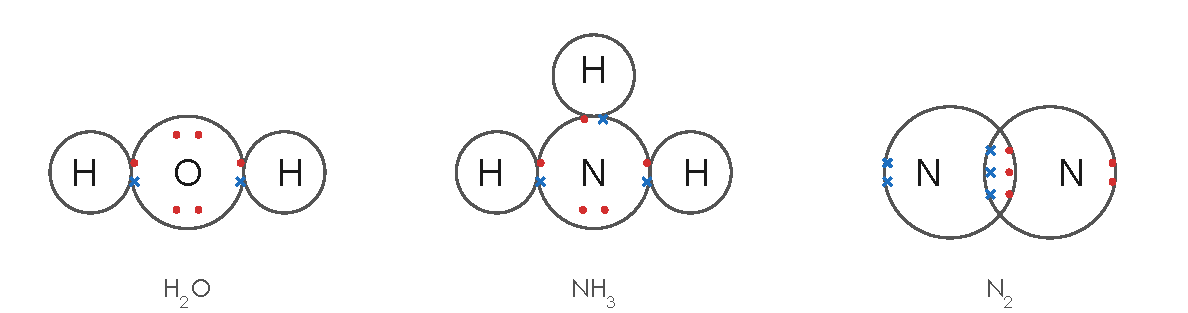
\includegraphics[width=0.62\textwidth]{images/UD4/lewis_H2O_NH3_N2}
    \caption{Pares compartidos en el agua, el amoníaco y el nitrógeno. En el \ch{N2} los átomos comparten tres pares.}
    \label{fig:ud4-H2O}
\end{figure}

\paragraph{Enlaces simples, dobles y triples.} Si los átomos comparten \textbf{un par} de electrones, el enlace es
\textbf{simple}; si comparten \textbf{dos}, es \textbf{doble}, y si comparten \textbf{tres}, \textbf{triple}:
\[ \chemfig{\charge{90=\:,180=\:,270=\:}{Cl}-\charge{0=\:,90=\:,270=\:}{Cl}} \qquad\qquad
\chemfig{\charge{90=\:,270=\:}{O}=\charge{90=\:,270=\:}{O}} \qquad\qquad
\chemfig{\charge{180=\:}{N}~\charge{0=\:}{N}} \]
Los enlaces múltiples son más cortos y más fuertes que los simples: la energía del enlace triple N\(\equiv\)N del nitrógeno es
\qty{945}{\kilo\joule\per\mol}, una de las más altas que se conocen, y por eso el \ch{N2} del aire es tan poco reactivo.

\paragraph{Enlace covalente dativo.} A veces los dos electrones del par compartido los aporta \textbf{uno solo} de los átomos, que
tiene un par solitario, y el otro átomo tiene un orbital vacío. Es lo que ocurre cuando el amoníaco capta un ion \ch{H+}, que no
tiene ningún electrón, y forma el ion amonio, \ch{NH4+} (figura~\ref{fig:ud4-dativo}). Una vez formado, el enlace dativo es igual
que los demás. A veces se dibuja como una flecha que va del átomo que aporta el par al que lo recibe.

\begin{figure}[H]
    \centering
    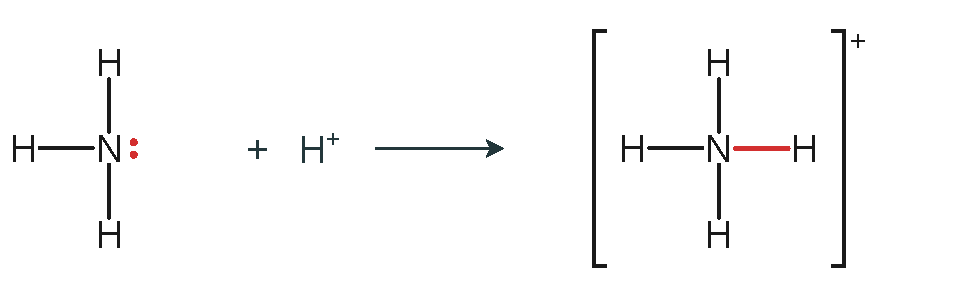
\includegraphics[width=0.55\textwidth]{images/UD4/dativo_amonio}
    \caption{Formación del ion amonio: el nitrógeno aporta los dos electrones del nuevo enlace (en rojo).}
    \label{fig:ud4-dativo}
\end{figure}

\subsection{Cómo escribir estructuras de Lewis}

Para moléculas sencillas, con un átomo central rodeado de otros, se puede seguir este método:
\begin{enumerate}[label=\numberballgreen]
    \item Se cuentan los electrones de valencia \textbf{disponibles}, \(D\), sumando los de todos los átomos (si es un ion, se
    suma un electrón por cada carga negativa o se resta uno por cada carga positiva).
    \item Se cuentan los electrones \textbf{necesarios}, \(N\), para que todos los átomos completen su capa: 8 por átomo y 2 por
    cada hidrógeno.
    \item Los electrones \textbf{compartidos} son \(C = N - D\), y el número de \textbf{enlaces} es \(C/2\).
    \item Se coloca en el centro el átomo menos electronegativo (nunca el H), se une a los demás con los enlaces calculados y se
    reparten los electrones restantes (\(D - C\)) como pares solitarios hasta completar los octetos.
\end{enumerate}

\begin{example}
    \textbf{Estructura de Lewis del \ch{CO2} y del \ch{HCN}.}

    \textbf{Solución.} \textbf{\ch{CO2}}: C (\conf{2s^2\,2p^2}) tiene 4 electrones de valencia y cada O (\conf{2s^2\,2p^4}), 6:
    \(D = 4 + 2 \cdot 6 = 16\). Necesarios: \(N = 3 \cdot 8 = 24\). Compartidos: \(C = 24 - 16 = 8\), es decir, \textbf{4
    enlaces}. El C va en el centro y forma un enlace doble con cada O; quedan \(16 - 8 = 8\) electrones, dos pares solitarios en
    cada O:
    \[ \chemfig{\charge{90=\:,270=\:}{O}=C=\charge{90=\:,270=\:}{O}} \]

    \textbf{\ch{HCN}}: \(D = 1 + 4 + 5 = 10\); \(N = 2 + 8 + 8 = 18\); \(C = 8\): \textbf{4 enlaces}. El C, en el centro, forma un
    enlace simple con el H y uno triple con el N; quedan \(10 - 8 = 2\) electrones, un par solitario en el N:
    \[ \chemfig{H-C~\charge{0=\:}{N}} \]
    Comprueba que el C tiene cuatro enlaces (valencia covalente 4), el N tres y el H uno.
\end{example}

\begin{example}
    \textbf{Formación de los enlaces del \ch{SCl2}.} Explica los enlaces del dicloruro de azufre.

    \textbf{Solución.} Escribimos las configuraciones electrónicas para ver cuántos electrones le faltan a cada átomo:
    S: \conf{[Ne]\,3s^2\,3p^4}, le faltan 2: valencia covalente 2. Cl: \conf{[Ne]\,3s^2\,3p^5}, le falta 1: valencia covalente 1.
    El azufre es el átomo central y comparte un par de electrones con cada cloro:
    \[ \chemfig{\charge{90=\:,180=\:,270=\:}{Cl}-\charge{90=\:,270=\:}{S}-\charge{0=\:,90=\:,270=\:}{Cl}} \]
\end{example}

\paragraph{Excepciones a la regla del octeto.} La regla del octeto falla en algunas moléculas (figura~\ref{fig:ud4-excepciones}):
\begin{itemize}
    \item \textbf{Octeto incompleto}: el boro y el aluminio, con 3 electrones de valencia, forman tres enlaces y se quedan con 6
    electrones (\ch{BF3}, \ch{BCl3}, \ch{AlCl3}); el berilio forma dos y se queda con 4 (\ch{BeCl2}).
    \item \textbf{Octeto expandido}: los elementos del tercer periodo y siguientes pueden rodearse de más de 8 electrones, porque
    disponen de orbitales \(d\) vacíos: el P en el \ch{PCl5} tiene 10 y el S en el \ch{SF6}, 12.
    \item \textbf{Número impar de electrones}: moléculas como el \ch{NO} (11 electrones de valencia) o el \ch{NO2} (17) tienen un
    electrón desapareado y no pueden completar el octeto de todos sus átomos. Se llaman \textbf{radicales} y son muy reactivas.
\end{itemize}

\begin{figure}[H]
    \centering
    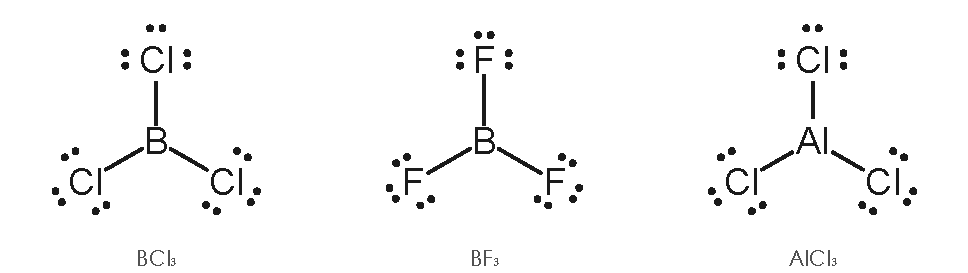
\includegraphics[width=0.45\textwidth]{images/UD4/octeto_incompleto}\hfill
    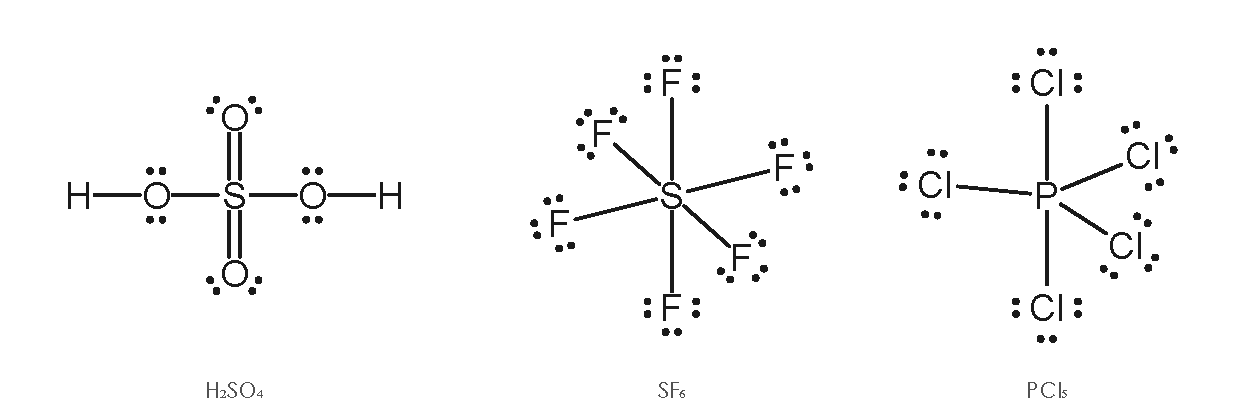
\includegraphics[width=0.45\textwidth]{images/UD4/octeto_ampliado}
    \caption{Excepciones a la regla del octeto: octeto incompleto (izquierda) y expandido (derecha).}
    \label{fig:ud4-excepciones}
\end{figure}

\paragraph{Energía y longitud de enlace.} La energía necesaria para romper un mol de enlaces covalentes en estado gaseoso es la
\textbf{energía de enlace}. Su valor depende de los átomos que se unen, pero en general es alto: el enlace covalente es un enlace
muy fuerte. Los enlaces dobles y triples son más fuertes y más cortos que los simples (tabla~\ref{tab:ud4-energias}).

\begin{table}[H]
    \centering
    \caption{Energía y longitud media de algunos enlaces covalentes}
    \vspace{-5pt}
    \begin{tabular}{@{}lcccccccc@{}}
        \toprule
        \textbf{Enlace} & H--H & C--H & O--H & C--C & C=C & C\(\equiv\)C & O=O & N\(\equiv\)N \\
        \midrule
        \textbf{Energía (\unit{\kilo\joule\per\mol})} & 436 & 413 & 463 & 347 & 614 & 839 & 498 & 945 \\[3pt]
        \textbf{Longitud (pm)} & 74 & 109 & 96 & 154 & 134 & 120 & 121 & 110 \\
        \bottomrule
    \end{tabular}
    \label{tab:ud4-energias}
\end{table}

\begin{exercise}
    Dibuja la estructura de Lewis del \ch{CO2}, el \ch{SiCl4} y el \ch{PH3}. Justifica en cada caso la valencia covalente de los
    átomos a partir de su configuración electrónica.
    \begin{solu}
        C: \conf{[He]\,2s^2\,2p^2}, valencia 4; O: \conf{[He]\,2s^2\,2p^4}, valencia 2;
        Si: \conf{[Ne]\,3s^2\,3p^2}, valencia 4; Cl: \conf{[Ne]\,3s^2\,3p^5}, valencia 1; P: \conf{[Ne]\,3s^2\,3p^3}, valencia 3;
        H: \conf{1s^1}, valencia 1.
        \begin{center}
            \textcolor{red}{\chemfig{\charge{90=\:,270=\:}{O}=C=\charge{90=\:,270=\:}{O}}} \qquad
            \textcolor{red}{\chemfig{Si(-[2]\charge{0=\:,90=\:,180=\:}{Cl})(-[4]\charge{90=\:,180=\:,270=\:}{Cl})(-[6]\charge{0=\:,180=\:,270=\:}{Cl})-\charge{0=\:,90=\:,270=\:}{Cl}}} \qquad
            \textcolor{red}{\chemfig{H-\charge{90=\:}{P}(-[6]H)-H}}
        \end{center}
    \end{solu}
\end{exercise}

\begin{exercise}
    Calcula, con el método de los electrones disponibles y necesarios, cuántos enlaces hay en el \ch{H2CO} (metanal) y dibuja su
    estructura de Lewis. ¿Qué tipo de enlace une el C con el O?
    \begin{solu}
        \(D = 2 \cdot 1 + 4 + 6 = 12\); \(N = 2 \cdot 2 + 8 + 8 = 20\); \(C = 8\): \textcolor{red}{4 enlaces}. El C, en el
        centro, se une a cada H con un enlace simple y al O con uno \textcolor{red}{doble}; quedan 4 electrones, dos pares
        solitarios en el O:
        \textcolor{red}{\chemfig{C(-[:150]H)(-[:210]H)=\charge{90=\:,270=\:}{O}}}.
    \end{solu}
\end{exercise}

\begin{exercise}
    El ion hidronio, \ch{H3O+}, se forma cuando una molécula de agua capta un ion \ch{H+}. Dibuja su estructura de Lewis e indica
    qué enlace es dativo y qué átomo aporta el par de electrones.
    \begin{solu}
        El oxígeno del agua tiene dos pares solitarios y \textcolor{red}{aporta uno de ellos} al \ch{H+}, que no tiene electrones:
        \textcolor{red}{el enlace O--H nuevo es dativo}. En el \ch{H3O+} el O tiene tres enlaces y un par solitario:
        \(\left[\,\chemfig{H-\charge{90=\:}{O}(-[6]H)-H}\,\right]^+\).
    \end{solu}
\end{exercise}

\begin{exercise}
    ¿Cumplen la regla del octeto el átomo central del \ch{BeF2}, del \ch{PF5} y del \ch{NO}? Justifícalo.
    \begin{solu}
        \textcolor{red}{No, ninguno.} \ch{BeF2}: el Be forma dos enlaces y queda con 4 electrones (octeto incompleto).
        \ch{PF5}: el P forma cinco enlaces y queda con 10 (octeto expandido, posible porque está en el periodo 3).
        \ch{NO}: tiene \(5 + 6 = 11\) electrones de valencia, un número impar: uno de los átomos queda con un electrón desapareado.
    \end{solu}
\end{exercise}

\subsection{Polaridad del enlace covalente}

Si los dos átomos que comparten electrones son \textbf{iguales} (\ch{H2}, \ch{Cl2}, \ch{O2}), atraen con la misma fuerza a los
electrones del enlace, que quedan repartidos por igual: la nube electrónica es \textbf{simétrica} y el enlace es \textbf{apolar}.

Si los átomos son \textbf{distintos}, el más \textbf{electronegativo} atrae con más intensidad a los electrones compartidos, y la
nube se desplaza hacia él. En el \ch{HCl}, el cloro (\(\mathrm{EN} = \num{3.2}\)) atrae el par más que el hidrógeno
(\(\mathrm{EN} = \num{2.2}\)): cerca del cloro hay un exceso de carga negativa, que se indica \(\delta^-\), y cerca del hidrógeno, un
déficit, \(\delta^+\). El enlace es \textbf{polar} y forma un pequeño \textbf{dipolo}:
\[ \overset{\delta^+}{\mathrm{H}}{-}\overset{\delta^-}{\mathrm{Cl}} \]

\begin{definition}[Polaridad del enlace]
    Un enlace covalente es \textbf{polar} cuando los átomos que lo forman tienen distinta electronegatividad. La polaridad es mayor
    cuanto mayor es la \textbf{diferencia de electronegatividad}, \(\Delta\mathrm{EN}\), y se mide con el \textbf{momento dipolar}
    del enlace, \(\vec{\mu} = q \cdot \vec{d}\): un vector dirigido a lo largo del enlace que, en química, apunta hacia el átomo
    más electronegativo. Se mide en debyes (D).
\end{definition}

La diferencia de electronegatividad sirve también para decidir el tipo de enlace. De forma orientativa:

\begin{table}[H]
    \centering
    \caption{Tipo de enlace según la diferencia de electronegatividad}
    \vspace{-5pt}
    \begin{tabular}{@{}lll@{}}
        \toprule
        \(\boldsymbol{\Delta}\textbf{EN}\) & \textbf{Tipo de enlace} & \textbf{Ejemplos} \\
        \midrule
        Hasta \num{0.4} & Covalente apolar (o casi) & \ch{H2} (0), \ch{Cl2} (0), \ch{C-H} (0,4) \\[3pt]
        De \num{0.5} a \num{1.7} & Covalente polar & \ch{HCl} (1,0), \ch{H2O} (O--H: 1,2), \ch{HF} (1,8) \\[3pt]
        Mayor que \num{1.7} & Iónico & \ch{NaCl} (2,3), \ch{KF} (3,2), \ch{MgO} (2,1) \\
        \bottomrule
    \end{tabular}
    \label{tab:ud4-den}
\end{table}

El paso de un tipo a otro es gradual (el \ch{HF}, con \(\Delta\mathrm{EN} = \num{1.8}\), es covalente polar). El enlace iónico
puede verse como el \textbf{caso extremo} del enlace covalente polar: la diferencia de electronegatividad es tan grande que el par
de electrones pasa por completo al no metal, como si el metal se lo hubiera cedido.

\begin{example}
    \textbf{Ordenar por polaridad.} Indica si son polares o apolares los enlaces del \ch{N2}, el \ch{HBr} y el \ch{CO}, y ordénalos
    de menor a mayor polaridad.

    \textbf{Solución.} En el \ch{N2} los dos átomos son iguales: \(\Delta\mathrm{EN} = 0\), enlace \textbf{apolar}. En el
    \ch{HBr}, \(\Delta\mathrm{EN} = \num{3.0} - \num{2.2} = \num{0.8}\), y en el \ch{CO}, \(\num{3.4} - \num{2.6} = \num{0.8}\):
    los dos son \textbf{polares}, con el polo negativo en el Br y en el O. Con estos valores tienen una polaridad parecida, y el
    orden es \(\ch{N2} < \ch{CO} \approx \ch{HBr}\).
\end{example}

\begin{exercise}
    Indica si son polares o apolares los enlaces de estas sustancias y clasifícalas según su \(\Delta\mathrm{EN}\): \ch{F2},
    \ch{HF}, \ch{NH3}, \ch{HI}, \ch{KCl} y \ch{CS2}.
    \begin{solu}
        \ch{F2}: 0, \textcolor{red}{covalente apolar}. \ch{HF}: 1,8, \textcolor{red}{covalente muy polar}. \ch{NH3} (N--H): 0,8,
        \textcolor{red}{covalente polar}. \ch{HI}: 0,5, \textcolor{red}{covalente poco polar}. \ch{KCl}: 2,4,
        \textcolor{red}{iónico}. \ch{CS2}: 0, \textcolor{red}{covalente apolar} (C y S tienen la misma EN, 2,6).
    \end{solu}
\end{exercise}

\begin{exercise}
    Dibuja las estructuras de Lewis del \ch{CH3Cl}, el \ch{C2H2} y el \ch{OF2}, e indica la polaridad de cada uno de sus enlaces.
    \begin{solu}
        \textcolor{red}{\chemfig{C(-[2]H)(-[4]H)(-[6]H)-\charge{0=\:,90=\:,270=\:}{Cl}}} \quad C--H poco polar (0,4); C--Cl polar
        (0,6), con el \(\delta^-\) en el Cl. \quad
        \textcolor{red}{\chemfig{H-C~C-H}} \quad C--H poco polar; el triple C\(\equiv\)C, apolar. \quad
        \textcolor{red}{\chemfig{\charge{90=\:,180=\:,270=\:}{F}-\charge{90=\:,270=\:}{O}-\charge{0=\:,90=\:,270=\:}{F}}} \quad
        O--F polar (0,6), con el \(\delta^-\) en el F.
    \end{solu}
\end{exercise}

%========================================================================================
\section{Sustancias covalentes moleculares}\label{sec:ud4-moleculares}
%========================================================================================

En la mayoría de las sustancias covalentes, unos pocos átomos se unen entre sí y forman una \textbf{molécula}: el agua (\ch{H2O}),
el oxígeno (\ch{O2}), el amoníaco (\ch{NH3}) o la glucosa (\ch{C6H12O6}) son sustancias \textbf{covalentes moleculares}. Su
\textbf{fórmula molecular} indica, además de la proporción, el número exacto de átomos de cada elemento que hay en cada molécula:
una molécula de glucosa tiene 6 átomos de carbono, 12 de hidrógeno y 6 de oxígeno.

\subsection{Geometría de las moléculas}

Las estructuras de Lewis indican qué átomos están unidos, pero no la forma de la molécula. Para predecirla se usa la
\textbf{teoría de repulsión de los pares de electrones de la capa de valencia} (TRPECV):

\begin{definition}[TRPECV]
    Los pares de electrones de la capa de valencia del átomo central, enlazantes y no enlazantes, se repelen y se colocan en el
    espacio \textbf{lo más alejados posible} unos de otros. Los pares no enlazantes ocupan más espacio que los enlazantes y cierran
    un poco los ángulos entre los enlaces. Un enlace doble o triple cuenta como una sola dirección.
\end{definition}

Primero se busca la distribución de \textbf{todos} los pares (geometría de los pares electrónicos) y luego se describe la forma de
la molécula mirando solo dónde están los \textbf{átomos} (geometría molecular):

\begin{table}[H]
    \centering
    \caption{Geometría de las moléculas según la TRPECV}
    \vspace{-5pt}
    \begin{tabular}{@{}cccL{3.2cm}cc@{}}
        \toprule
        \makecell{\textbf{Pares en} \\ \textbf{el átomo central}} & \textbf{Enlazantes} & \textbf{Solitarios} &
        \textbf{Geometría molecular} & \textbf{Ángulo} & \textbf{Ejemplos} \\
        \midrule
        2 & 2 & 0 & Lineal & \ang{180} & \ch{BeCl2}, \ch{CO2} \\[3pt]
        3 & 3 & 0 & Triangular plana & \ang{120} & \ch{BF3}, \ch{SO3} \\[3pt]
        3 & 2 & 1 & Angular & \(< \ang{120}\) & \ch{SO2}, \ch{O3} \\[3pt]
        4 & 4 & 0 & Tetraédrica & \ang{109.5} & \ch{CH4}, \ch{CCl4} \\[3pt]
        4 & 3 & 1 & Pirámide trigonal & \(\approx \ang{107}\) & \ch{NH3}, \ch{PCl3} \\[3pt]
        4 & 2 & 2 & Angular & \(\approx \ang{104.5}\) & \ch{H2O}, \ch{H2S} \\
        \bottomrule
    \end{tabular}
    \label{tab:ud4-trpecv}
\end{table}

\begin{figure}[H]
    \centering
    \begin{minipage}{0.32\textwidth}\centering 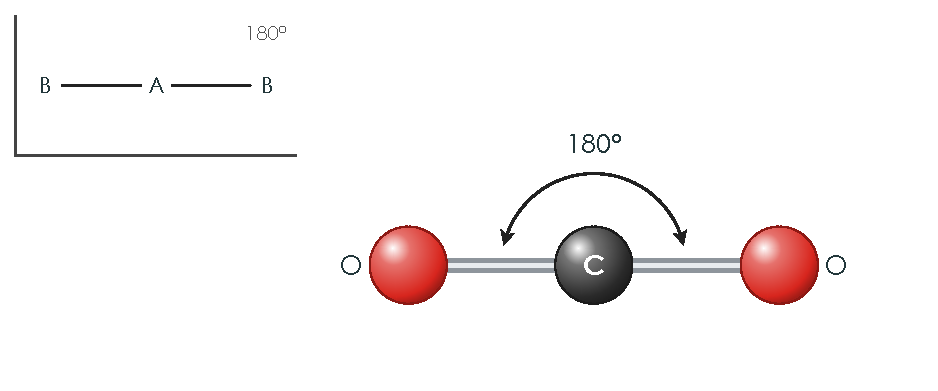
\includegraphics[width=\linewidth,height=2.8cm,keepaspectratio]{images/UD4/geo_lineal}\\ \small Lineal (\ch{CO2})\end{minipage}\hfill
    \begin{minipage}{0.32\textwidth}\centering 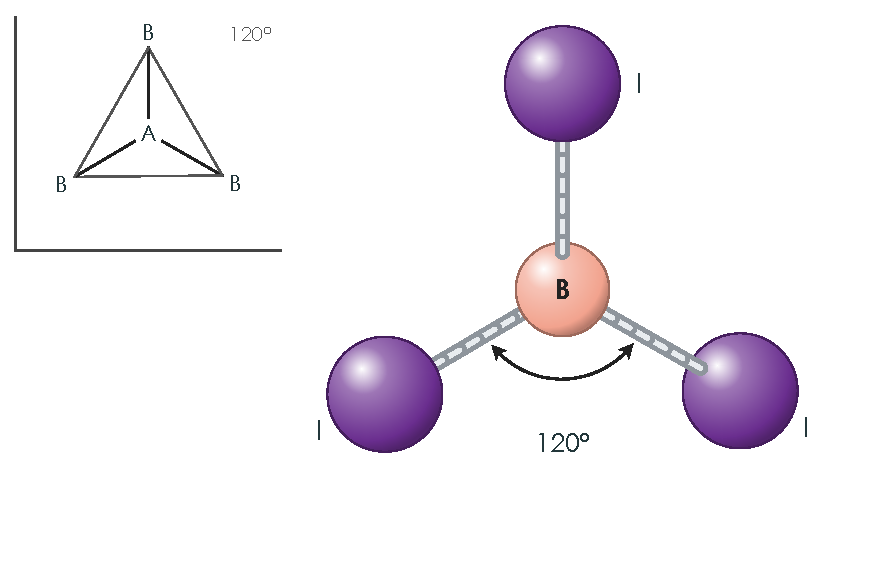
\includegraphics[width=\linewidth,height=2.8cm,keepaspectratio]{images/UD4/geo_trigonal}\\ \small Triangular plana (\ch{BI3})\end{minipage}\hfill
    \begin{minipage}{0.32\textwidth}\centering 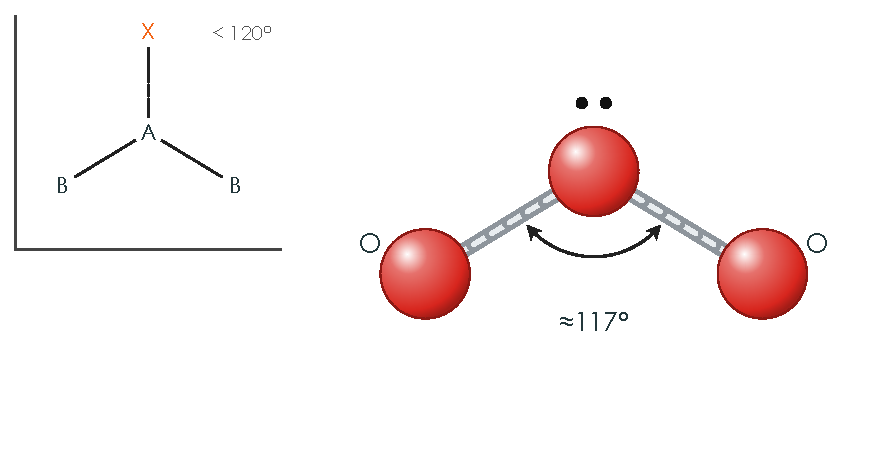
\includegraphics[width=\linewidth,height=2.8cm,keepaspectratio]{images/UD4/geo_angular3}\\ \small Angular, 1 par solitario (\ch{O3})\end{minipage}
    \\[8pt]
    \begin{minipage}{0.32\textwidth}\centering 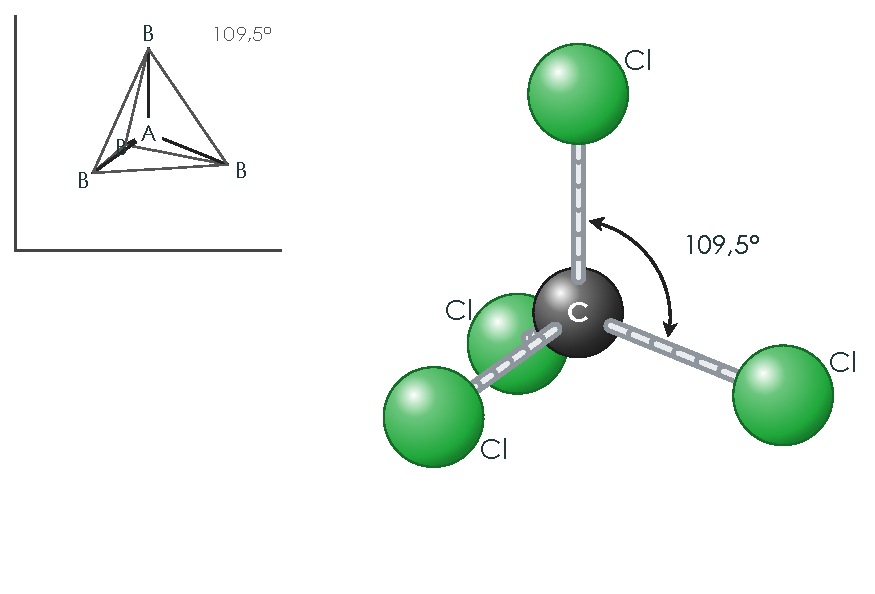
\includegraphics[width=\linewidth,height=2.8cm,keepaspectratio]{images/UD4/geo_tetraedrica}\\ \small Tetraédrica (\ch{CCl4})\end{minipage}\hfill
    \begin{minipage}{0.32\textwidth}\centering 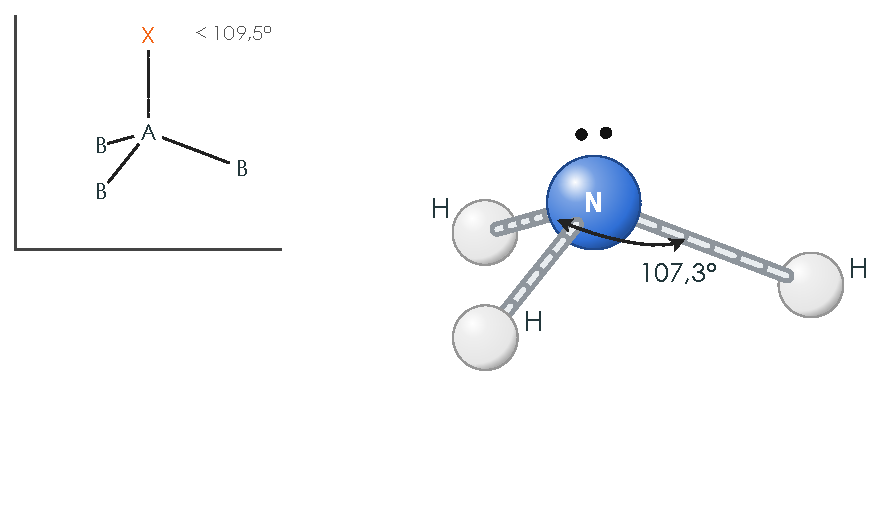
\includegraphics[width=\linewidth,height=2.8cm,keepaspectratio]{images/UD4/geo_piramidal}\\ \small Pirámide trigonal (\ch{NH3})\end{minipage}\hfill
    \begin{minipage}{0.32\textwidth}\centering 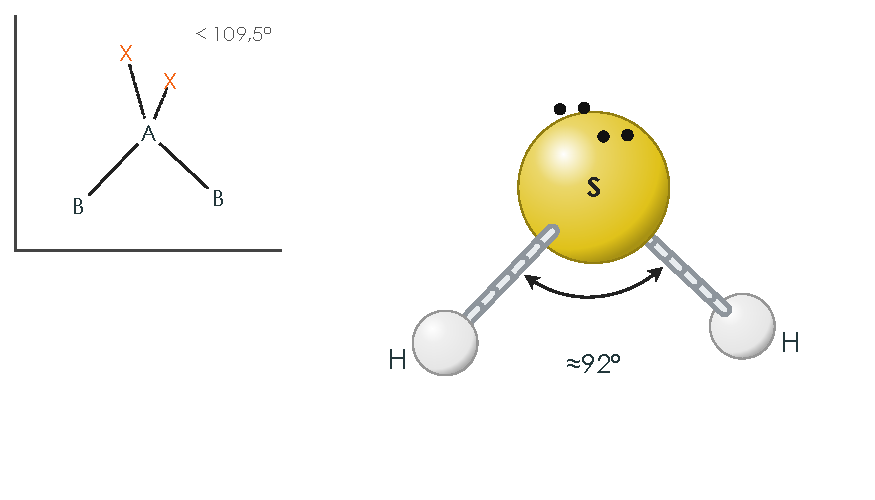
\includegraphics[width=\linewidth,height=2.8cm,keepaspectratio]{images/UD4/geo_angular4}\\ \small Angular, 2 pares solitarios (\ch{H2S})\end{minipage}
    \caption{Geometrías moleculares más sencillas. En cada una, a la izquierda, el esquema con el átomo central A, los átomos
    enlazados B y los pares solitarios X.}
    \label{fig:ud4-geometrias}
\end{figure}

\begin{example}
    \textbf{Geometría del agua.} ¿Por qué la molécula de agua es angular y no lineal?

    \textbf{Solución.} El oxígeno del agua tiene \textbf{cuatro} pares de electrones en su capa de valencia: dos enlazantes (con
    los H) y dos solitarios. Los cuatro pares se dirigen hacia los vértices de un tetraedro; como solo dos de ellos tienen átomo,
    la molécula es \textbf{angular}. Los pares solitarios repelen con más fuerza y cierran el ángulo H--O--H desde
    \ang{109.5} hasta \ang{104.5} (figura~\ref{fig:ud4-repulsiones}).
\end{example}

\begin{figure}[H]
    \centering
    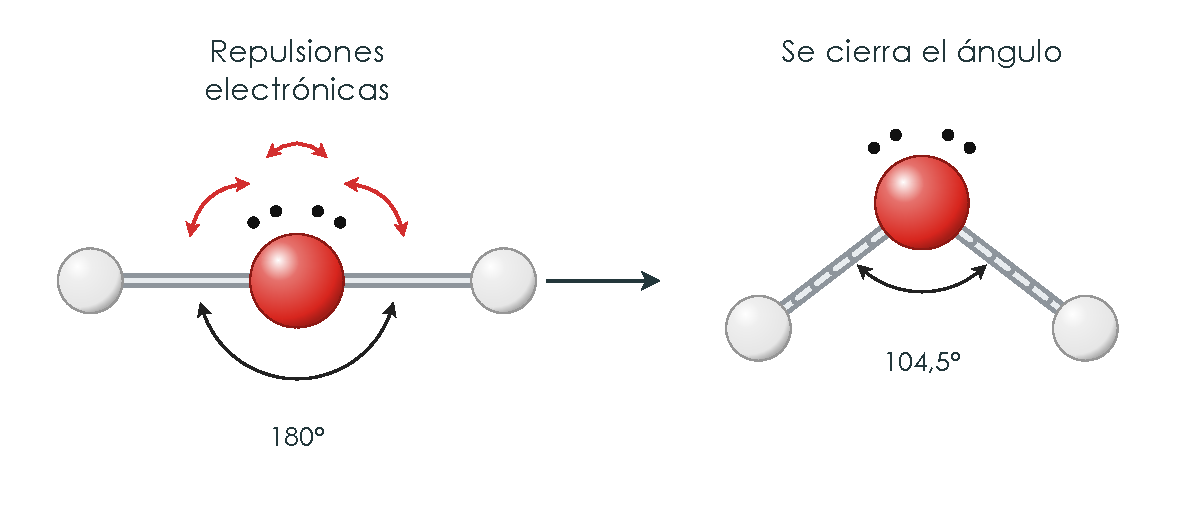
\includegraphics[width=0.55\textwidth]{images/UD4/repulsiones}
    \caption{Los pares solitarios del oxígeno repelen a los enlaces y la molécula de agua se dobla.}
    \label{fig:ud4-repulsiones}
\end{figure}

\subsection{Polaridad de las moléculas}

Una molécula es \textbf{polar} cuando tiene una zona con más densidad de carga negativa y otra con menos: se comporta como un
dipolo. Que lo sea depende de sus \textbf{enlaces} y de su \textbf{geometría}.

\begin{definition}[Momento dipolar de una molécula]
    Es la \textbf{suma vectorial} de los momentos dipolares de todos sus enlaces.
    \begin{itemize}
        \item Si todos los enlaces son apolares, la molécula es \textbf{apolar} (\ch{H2}, \ch{Cl2}).
        \item Si tiene enlaces polares, puede ser \textbf{polar} o \textbf{apolar}: si la molécula es simétrica, los momentos de los
        enlaces se anulan y es apolar (\(\vec{\mu} = 0\)); si no, es polar (\(\vec{\mu} \neq 0\)).
    \end{itemize}
\end{definition}

\begin{figure}[H]
    \centering
    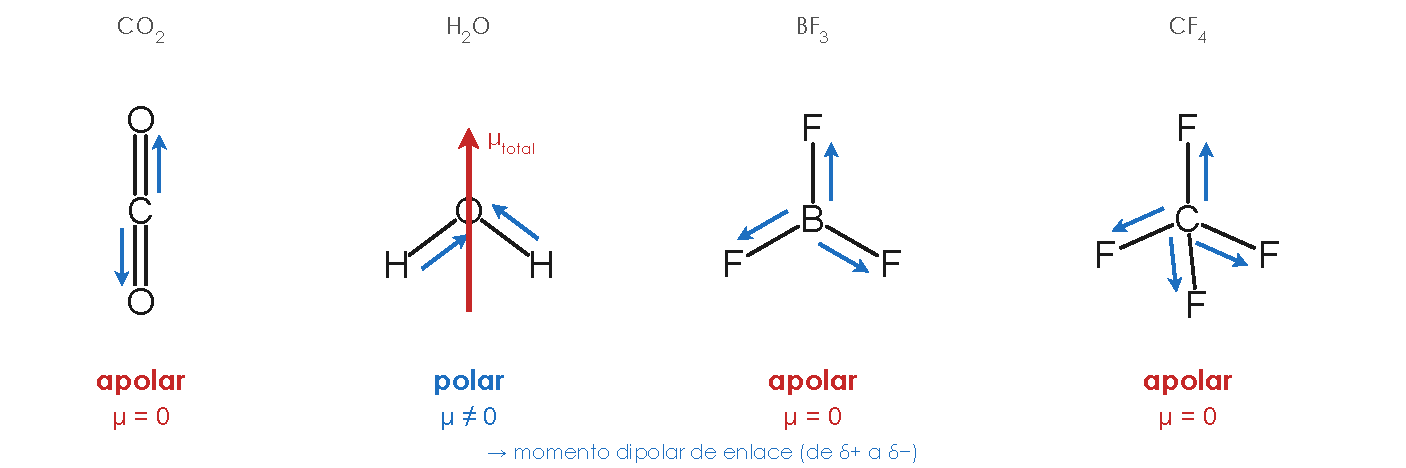
\includegraphics[width=0.75\textwidth]{images/UD4/polaridad_moleculas}
    \caption{El \ch{CO2}, el \ch{BF3} y el \ch{CF4} tienen enlaces polares pero son simétricos: sus momentos se anulan. El agua,
    angular, es polar.}
    \label{fig:ud4-polaridad}
\end{figure}

Por ejemplo, el \ch{CO2} y el \ch{CF4} tienen enlaces polares, pero por su simetría (lineal y tetraédrica) son
\textbf{apolares}; el \ch{H2O} (angular), el \ch{NH3} (piramidal) y el \ch{CH3F} (tetraédrica, pero con un átomo distinto) son
\textbf{polares} (figura~\ref{fig:ud4-polaridad}).

\begin{exercise}
    Predice la geometría y la polaridad de estas moléculas: a) \ch{BCl3}; b) \ch{PH3}; c) \ch{SiH4}; d) \ch{H2S}; e) \ch{CHCl3}.
    \begin{solu}
        a) 3 pares enlazantes: \textcolor{red}{triangular plana, apolar}. b) 3 enlazantes y 1 solitario:
        \textcolor{red}{pirámide trigonal, polar}. c) 4 enlazantes: \textcolor{red}{tetraédrica, apolar}. d) 2 enlazantes y 2
        solitarios: \textcolor{red}{angular, polar}. e) 4 enlazantes, pero un H y tres Cl: \textcolor{red}{tetraédrica
        (deformada), polar}: los momentos de los enlaces no se anulan.
    \end{solu}
\end{exercise}

\begin{exercise}
    El \ch{BF3} y el \ch{NF3} tienen fórmulas parecidas. Sin embargo, el primero es apolar y el segundo, polar. Explícalo.
    \begin{solu}
        El B tiene 3 electrones de valencia y forma 3 enlaces sin pares solitarios: \textcolor{red}{\ch{BF3} es triangular plana}
        y los tres momentos de enlace, iguales y a \ang{120}, se anulan. El N tiene 5: forma 3 enlaces y le queda un par
        solitario: \textcolor{red}{\ch{NF3} es una pirámide trigonal} y los momentos no se anulan.
    \end{solu}
\end{exercise}

\subsection{Fuerzas intermoleculares}

El \textbf{estado físico} de una sustancia depende de la intensidad de las fuerzas entre sus partículas. Que una sustancia
covalente molecular pueda ser sólida o líquida demuestra que sus \textbf{moléculas se atraen entre sí}.

\begin{remark}
    \textbf{Intra- e intermolecular.} Los enlaces covalentes unen a los átomos \textbf{dentro} de la molécula: son fuerzas
    \textbf{intra}moleculares, muy intensas. Las fuerzas \textbf{inter}moleculares actúan \textbf{entre} moléculas distintas y son
    mucho más débiles. Al hervir agua no se rompen las moléculas de \ch{H2O}: solo se separan unas de otras.
\end{remark}

Las fuerzas intermoleculares, que a veces se llaman en conjunto \textbf{fuerzas de Van der Waals}, son de tres tipos, y su
intensidad depende sobre todo de la polaridad de las moléculas:

\paragraph{Fuerzas dipolo-dipolo.} Una molécula \textbf{polar} es un dipolo permanente: la parte negativa de una molécula atrae a
la parte positiva de la vecina (figura~\ref{fig:ud4-dipolo}). Se dan, por ejemplo, entre las moléculas de \ch{HCl} o de
\ch{H2S}.

\begin{figure}[H]
    \centering
    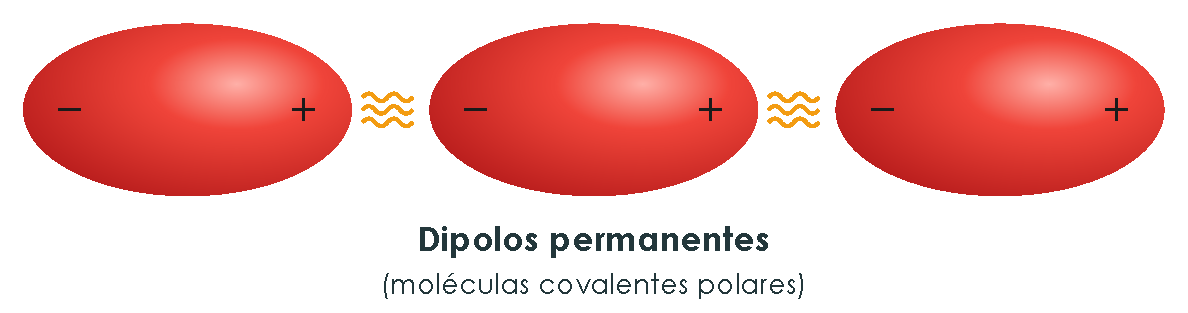
\includegraphics[width=0.6\textwidth]{images/UD4/dipolo_dipolo}
    \caption{Fuerzas dipolo-dipolo entre moléculas polares.}
    \label{fig:ud4-dipolo}
\end{figure}

\paragraph{Fuerzas de dispersión (o de London).} Incluso en las moléculas \textbf{apolares}, el movimiento continuo de los
electrones hace que, en un instante dado, haya más carga negativa en un extremo que en otro: se forma un \textbf{dipolo
instantáneo}, que a su vez deforma la nube de la molécula vecina y crea en ella un \textbf{dipolo inducido}
(figura~\ref{fig:ud4-dispersion}). Las dos se atraen durante un instante. Son fuerzas muy débiles, pero existen entre
\textbf{todas} las moléculas, y son tanto más intensas cuanto \textbf{mayor} es la molécula: tiene más electrones y su nube es
más fácil de deformar. Por eso, a temperatura ambiente, el \ch{F2} y el \ch{Cl2} son gases, el \ch{Br2} es líquido y el \ch{I2},
sólido.

\begin{figure}[H]
    \centering
    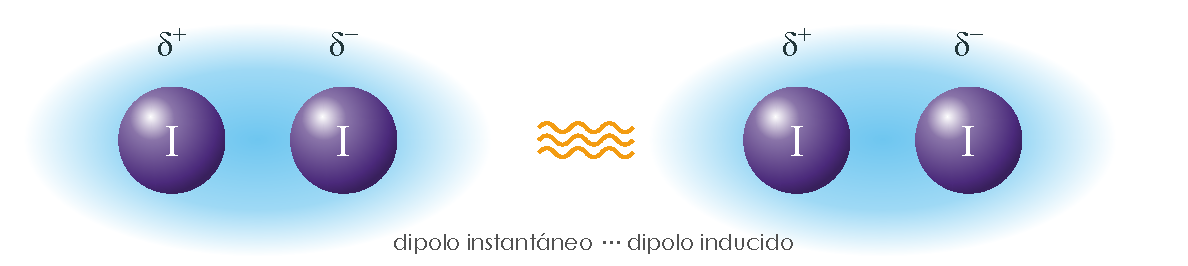
\includegraphics[width=0.6\textwidth]{images/UD4/dispersion}
    \caption{Fuerzas de dispersión: un dipolo instantáneo induce otro en la molécula vecina.}
    \label{fig:ud4-dispersion}
\end{figure}

\paragraph{Enlace (o puente) de hidrógeno.} Cuando el hidrógeno está unido a un átomo \textbf{muy electronegativo y pequeño}
(\textbf{F}, \textbf{O} o \textbf{N}), el enlace es muy polar y el H queda casi «desnudo», con una carga positiva parcial
grande. Ese H es atraído con fuerza por un par solitario del F, O o N de una molécula vecina (figura~\ref{fig:ud4-puentes}).
Es la fuerza intermolecular más intensa, aunque sigue siendo unas diez veces más débil que un enlace covalente. Se da en el
\ch{HF}, el \ch{H2O}, el \ch{NH3}, los alcoholes o el ADN, cuyas dos hebras se mantienen unidas por puentes de hidrógeno.

\begin{figure}[H]
    \centering
    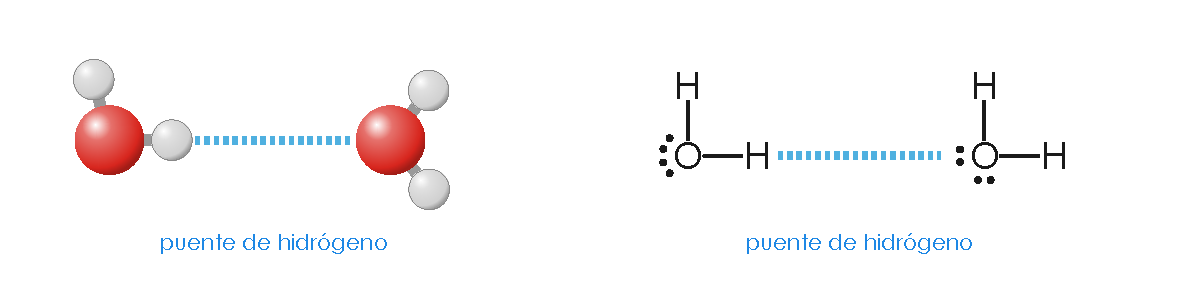
\includegraphics[width=0.6\textwidth]{images/UD4/puentes_H_agua}
    \caption{Enlace de hidrógeno entre dos moléculas de agua.}
    \label{fig:ud4-puentes}
\end{figure}

Los enlaces de hidrógeno explican por qué el agua es líquida a temperatura ambiente cuando las sustancias parecidas a ella (\ch{H2S},
\ch{H2Se}, \ch{H2Te}) son gases: si no fuera por ellos, el agua herviría a unos \qty{-80}{\degreeCelsius}
(figura~\ref{fig:ud4-hidruros}). Lo mismo les ocurre al \ch{HF} y al \ch{NH3} en sus grupos. En el grupo 14, cuyos hidruros son
apolares, el punto de ebullición sube regularmente con el tamaño de la molécula.

\begin{figure}[H]
    \centering
    \begin{tikzpicture}
        \begin{axis}[grafica, width=0.7\linewidth, height=6.2cm,
            xmin=1.7, xmax=5.3, ymin=-180, ymax=120, xtick={2,3,4,5}, xlabel={Periodo},
            ylabel={Temperatura de ebullición (\unit{\degreeCelsius})}, ytick={-150,-100,-50,0,50,100},
            legend style={font=\scriptsize, at={(1.02,0.5)}, anchor=west, draw=none}, legend cell align=left]
            \addplot[thick, mark=*, red!70!black] coordinates {(2,100) (3,-60.3) (4,-41.3) (5,-2)};
            \addplot[thick, mark=square*, ocre] coordinates {(2,19.5) (3,-85) (4,-66.8) (5,-35.4)};
            \addplot[thick, mark=triangle*, blue!70!black] coordinates {(2,-33.3) (3,-87.7) (4,-62.5) (5,-17)};
            \addplot[thick, mark=diamond*, gray] coordinates {(2,-161.5) (3,-111.9) (4,-88.5) (5,-52)};
            \legend{Grupo 16: \ch{H2O} \dots\ \ch{H2Te}, Grupo 17: \ch{HF} \dots\ \ch{HI}, Grupo 15: \ch{NH3} \dots\ \ch{SbH3},
                Grupo 14: \ch{CH4} \dots\ \ch{SnH4}}
        \end{axis}
    \end{tikzpicture}
    \caption{Temperatura de ebullición de los hidruros de los grupos 14 a 17. El \ch{H2O}, el \ch{HF} y el \ch{NH3} se salen de
    la tendencia por los enlaces de hidrógeno.}
    \label{fig:ud4-hidruros}
\end{figure}

\subsection{Propiedades de las sustancias covalentes moleculares}

\begin{itemize}
    \item A temperatura ambiente pueden ser gases (\ch{O2}, \ch{CO2}), líquidos (agua, etanol) o sólidos (yodo, azúcar), pero todas
    tienen \textbf{puntos de fusión y ebullición bajos}, porque solo hay que vencer las débiles fuerzas intermoleculares.
    \item En estado sólido son \textbf{blandas} y \textbf{frágiles}, por la misma razón.
    \item \textbf{No conducen la electricidad}: los electrones están localizados en los enlaces y no hay cargas libres.
    \item Su \textbf{solubilidad} depende de su polaridad, según la regla «lo semejante disuelve a lo semejante»: las sustancias
    \textbf{polares} se disuelven en disolventes polares, como el agua, y las \textbf{apolares}, en disolventes apolares, como la
    gasolina, el tetracloruro de carbono o el hexano.
\end{itemize}

\begin{example}
    \textbf{¿Por qué el agua es líquida y el dióxido de carbono, gas?} A temperatura ambiente, el agua (\(M = \qty{18}{\gram\per\mol}\))
    es líquida, mientras que el \ch{CO2} (\(M = \qty{44}{\gram\per\mol}\)) es un gas. Explícalo.

    \textbf{Solución.} Las dos son sustancias covalentes moleculares, así que su estado depende de las fuerzas entre sus moléculas.
    El \ch{CO2} es lineal y \textbf{apolar}: entre sus moléculas solo hay fuerzas de dispersión, débiles. El agua es angular y muy
    \textbf{polar}, y sus moléculas, con H unidos a O, forman \textbf{enlaces de hidrógeno}, mucho más intensos. Aunque la
    molécula de \ch{CO2} es mayor, separar las moléculas de agua cuesta mucha más energía: el agua hierve a
    \qty{100}{\degreeCelsius} y el \ch{CO2} sublima a \qty{-78}{\degreeCelsius}.
\end{example}

\begin{exercise}
    ¿Cuáles de estas sustancias serán solubles en agua? a) \ch{CH3OH} (metanol); b) \ch{N2}; c) \ch{KBr}; d) \ch{C8H18} (octano);
    e) \ch{NH3}; f) \ch{Cl2}; g) sacarosa, \ch{C12H22O11}.
    \begin{solu}
        Solubles: \textcolor{red}{a) metanol, c) \ch{KBr}, e) \ch{NH3} y g) sacarosa}: el \ch{KBr} es iónico, y el metanol, el
        amoníaco y la sacarosa son polares y forman enlaces de hidrógeno con el agua. \textcolor{red}{Poco o nada solubles: b),
        d) y f)}, que son apolares.
    \end{solu}
\end{exercise}

\begin{exercise}
    ¿Qué fuerzas intermoleculares hay entre las moléculas de cada una de estas sustancias? a) \ch{CH4}; b) \ch{HBr}; c) \ch{NH3};
    d) \ch{I2}; e) \ch{CH3CH2OH} (etanol).
    \begin{solu}
        a) \textcolor{red}{Solo de dispersión} (apolar). b) \textcolor{red}{Dipolo-dipolo y de dispersión}. c) \textcolor{red}{Enlaces
        de hidrógeno} (H unido a N), además de dipolo-dipolo y dispersión. d) \textcolor{red}{De dispersión}; como la molécula es
        grande, son bastante intensas y el yodo es sólido. e) \textcolor{red}{Enlaces de hidrógeno} (grupo O--H), dipolo-dipolo y
        dispersión.
    \end{solu}
\end{exercise}

\begin{exercise}
    Ordena de menor a mayor punto de ebullición: \ch{Cl2}, \ch{F2}, \ch{I2} y \ch{Br2}. ¿Qué fuerzas intermoleculares lo explican?
    \begin{solu}
        Son moléculas apolares y entre ellas solo hay \textcolor{red}{fuerzas de dispersión}, que aumentan con el tamaño (el número
        de electrones) de la molécula: \textcolor{red}{\(\ch{F2} < \ch{Cl2} < \ch{Br2} < \ch{I2}\)} (\(-188\), \(-34\), 59 y
        \qty{184}{\degreeCelsius}).
    \end{solu}
\end{exercise}

%========================================================================================
\section{Cristales covalentes}\label{sec:ud4-cristales}
%========================================================================================

En algunas sustancias, como el \textbf{diamante} y el \textbf{grafito} (dos formas del carbono) o la \textbf{sílice} (\ch{SiO2},
el cuarzo), los átomos se unen por enlaces covalentes formando \textbf{redes gigantes} en lugar de moléculas. Los átomos se
ordenan geométricamente en el espacio, así que estas sustancias tienen estructura \textbf{cristalina}: son \textbf{cristales
covalentes} (o sólidos covalentes).

\begin{itemize}
    \item En el \textbf{diamante}, cada átomo de carbono está unido a otros \textbf{cuatro} por enlaces covalentes, dirigidos
    hacia los vértices de un tetraedro, y la red se extiende en las tres direcciones (figura~\ref{fig:ud4-carbono}).
    \item En el \textbf{grafito}, cada carbono se une a otros \textbf{tres}, y forman \textbf{láminas} planas de hexágonos. Las
    láminas se apilan unas sobre otras unidas solo por fuerzas de dispersión, débiles, y el cuarto electrón de cada carbono queda
    deslocalizado por la lámina. Una sola lámina de grafito es el \textbf{grafeno}.
    \item En el \textbf{cuarzo}, cada átomo de silicio está unido a cuatro de oxígeno, y cada oxígeno a dos de silicio.
\end{itemize}

\begin{figure}[H]
    \centering
    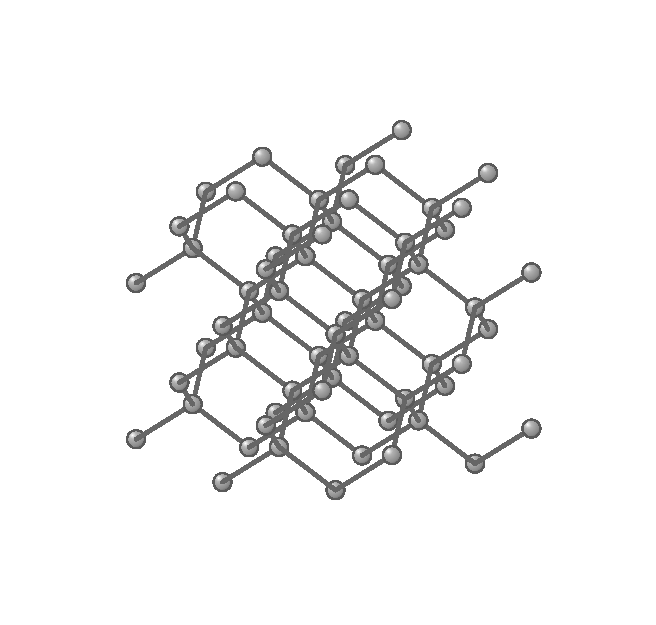
\includegraphics[width=0.4\textwidth]{images/UD4/diamante}\hspace{1cm}
    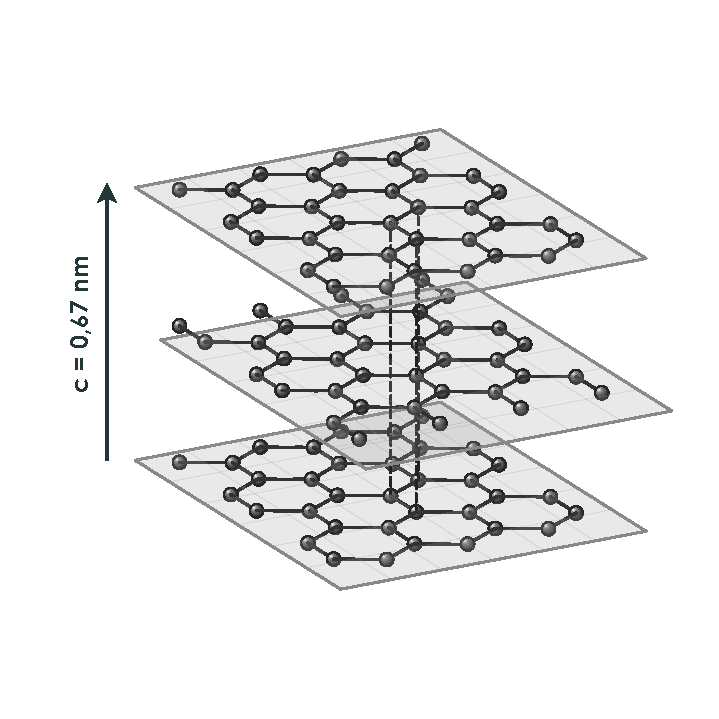
\includegraphics[width=0.4\textwidth]{images/UD4/grafito}
    \caption{Estructura del diamante (izquierda) y del grafito (derecha), con sus láminas separadas \qty{0.335}{\nm}.}
    \label{fig:ud4-carbono}
\end{figure}

\paragraph{Propiedades de los cristales covalentes.} Se deben a que el enlace covalente es el más fuerte de todos y a que, para
fundir o rayar el cristal, hay que romper un número enorme de enlaces:
\begin{itemize}
    \item Son \textbf{sólidos} con \textbf{puntos de fusión altísimos}, de miles de grados (el diamante se transforma a unos
    \qty{3550}{\degreeCelsius}; el cuarzo funde a \qty{1713}{\degreeCelsius}).
    \item Son \textbf{muy duros}: el diamante, con un 10 en la escala de Mohs, es la sustancia natural más dura.
    \item Sin embargo, son \textbf{frágiles}: los enlaces tienen direcciones fijas y se rompen si un golpe deforma la red.
    \item \textbf{No conducen la electricidad}, porque los electrones están localizados en los enlaces. La excepción es el
    \textbf{grafito}, que conduce a lo largo de sus láminas gracias a los electrones deslocalizados.
    \item Son \textbf{insolubles} en todos los disolventes.
\end{itemize}

\begin{remark}
    \textbf{El cristal de las ventanas no es un cristal.} El vidrio está hecho, sobre todo, de sílice, como el cuarzo, pero sus
    átomos están colocados de forma \textbf{desordenada}: no tiene estructura cristalina, sino \textbf{amorfa}. Por eso no funde a una
    temperatura fija, sino que se va reblandeciendo poco a poco, lo que permite soplarlo y moldearlo.
\end{remark}

\begin{example}
    \textbf{Diamante y grafito.} Si el diamante y el grafito están formados solo por átomos de carbono, ¿por qué el diamante es la
    sustancia natural más dura y el grafito es tan blando que se usa en las minas de los lápices?

    \textbf{Solución.} La diferencia está en cómo se unen los átomos. En el diamante, cada carbono forma cuatro enlaces covalentes
    con otros cuatro, en una red tridimensional: para rayarlo hay que romper enlaces covalentes en todas las direcciones. En el
    grafito, los átomos forman láminas unidas entre sí solo por fuerzas de dispersión: las láminas se deslizan unas sobre otras con
    facilidad y se quedan pegadas en el papel al escribir.
\end{example}

\begin{exercise}
    Busca información sobre otro cristal covalente (el carburo de silicio, el nitruro de boro o el propio cuarzo): su estructura,
    sus propiedades y sus usos. Compáralo con el diamante.
    \begin{solu}
        \textcolor{red}{Respuesta abierta.} Por ejemplo, el \textcolor{red}{carburo de silicio, \ch{SiC}} (carborundo), tiene una
        estructura como la del diamante con átomos de Si y C alternados; tiene una dureza de 9,5, funde a unos
        \qty{2700}{\degreeCelsius} y se usa en lijas, discos de corte, frenos cerámicos y en electrónica de potencia (es
        semiconductor). Es algo menos duro que el diamante pero más barato y resistente a la oxidación.
    \end{solu}
\end{exercise}

\begin{exercise}
    ¿Por qué el grafito conduce la electricidad y el diamante no? ¿En qué dirección conduce mejor el grafito?
    \begin{solu}
        \textcolor{red}{En el grafito, cada carbono usa solo tres electrones en enlaces y el cuarto queda deslocalizado por la
        lámina}; en el diamante los cuatro están localizados en enlaces. El grafito conduce mucho mejor
        \textcolor{red}{en la dirección de las láminas} que perpendicularmente a ellas.
    \end{solu}
\end{exercise}

%========================================================================================
\section{Propiedades de las sustancias}\label{sec:ud4-propiedades}
%========================================================================================

Según el tipo de enlace y las partículas que las forman, las sustancias se pueden clasificar en cuatro grupos
(figura~\ref{fig:ud4-tipos-sustancias}), con propiedades muy diferentes (tabla~\ref{tab:ud4-propiedades}).

\begin{figure}[H]
    \centering
    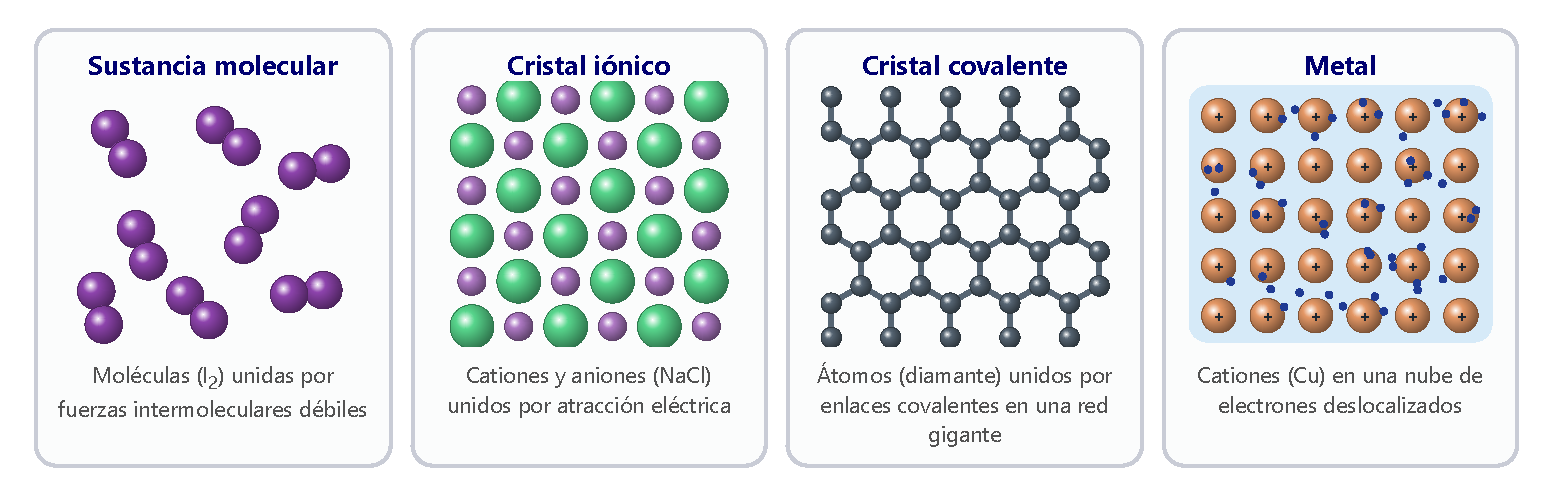
\includegraphics[width=\textwidth]{images/UD4/tipos_sustancias}
    \caption{Las cuatro clases de sustancias según su enlace.}
    \label{fig:ud4-tipos-sustancias}
\end{figure}

\begin{table}[H]
    \centering
    \caption{Propiedades de las sustancias según su tipo de enlace}
    \vspace{-5pt}
    \small
    \begin{tabular}{@{}L{2.25cm}L{2.7cm}L{2.7cm}L{2.7cm}L{2.7cm}@{}}
        \toprule
        & \textbf{Molecular} & \textbf{Metálica} & \textbf{Iónica} & \textbf{Cristal covalente} \\
        \midrule
        \textbf{Partículas} & Moléculas unidas por fuerzas intermoleculares & Cationes en una nube de electrones & Cationes y
        aniones & Átomos \\[3pt]
        \textbf{Fusión y ebullición} & Bajas & Variables (casi todos sólidos) & Altas & Muy altas \\[3pt]
        \textbf{Conductividad} & No conducen & Conducen muy bien & Solo fundidos o disueltos & No conducen (salvo el grafito) \\[3pt]
        \textbf{Dureza} & Blandas y frágiles & Tenaces, dúctiles y maleables & Duros pero frágiles & Muy duros pero frágiles \\[3pt]
        \textbf{Solubilidad} & Polares en polares; apolares en apolares & Insolubles (forman aleaciones) & Solubles en disolventes
        polares & Insolubles \\
        \bottomrule
    \end{tabular}
    \label{tab:ud4-propiedades}
\end{table}

\begin{example}
    \textbf{Identificar el enlace por las propiedades.} Una sustancia blanca funde a \qty{1074}{\degreeCelsius}, se disuelve en
    agua y su disolución conduce la electricidad, pero el sólido no. Otra, también blanca, funde a \qty{186}{\degreeCelsius}, se
    disuelve en agua y su disolución no conduce. ¿Qué tipo de sustancia es cada una?

    \textbf{Solución.} La primera tiene un punto de fusión alto y conduce solo disuelta, cuando sus iones quedan libres: es un
    \textbf{compuesto iónico} (puede ser el \ch{KCl}, que funde a \qty{770}{\degreeCelsius}, o el \ch{NaF}). La segunda funde a
    baja temperatura y no da iones en disolución: es una \textbf{sustancia covalente molecular} y, como se disuelve en agua,
    \textbf{polar} (puede ser la glucosa).
\end{example}

\subsection{Materiales de interés estratégico}

Un teléfono móvil contiene unos 40 elementos químicos distintos. Algunos materiales, como el \textbf{grafito}, el
\textbf{cobalto}, el \textbf{litio} o las \textbf{tierras raras}, se han vuelto imprescindibles para fabricar baterías, chips,
pantallas, imanes de motores eléctricos, aerogeneradores o placas solares, y su demanda no deja de crecer. Se consideran
\textbf{materiales de interés estratégico}, porque de ellos dependen sectores clave como la movilidad eléctrica, la producción de
energía o la defensa de un país.

El problema es que sus yacimientos están concentrados en muy pocos lugares, y su suministro se ve afectado por guerras,
conflictos comerciales o crisis como la de la pandemia de COVID-19. Un ejemplo es el \textbf{coltán}, una mezcla de los minerales
columbita y tantalita de la que se extrae el tántalo, con el que se fabrican condensadores diminutos. Gran parte procede de la
República Democrática del Congo, donde su extracción ha financiado conflictos armados y se hace a menudo en condiciones
durísimas.

Las soluciones pasan por \textbf{investigar} nuevos materiales, más abundantes, que sustituyan a los escasos, y por la
\textbf{economía circular}: alargar la vida de los aparatos, repararlos, reutilizarlos y, al final, reciclarlos para recuperar
sus materiales.

\begin{exercise}
    Para las sustancias \ch{LiBr}, \ch{Ag}, \ch{N2} y \ch{SiO2}: a) indica el tipo de enlace de cada una; b) ¿cuáles conducen la
    electricidad y en qué condiciones?; c) ¿cuáles son solubles en agua?
    \begin{solu}
        a) \ch{LiBr}: \textcolor{red}{iónico}; \ch{Ag}: \textcolor{red}{metálico}; \ch{N2}: \textcolor{red}{covalente molecular};
        \ch{SiO2}: \textcolor{red}{cristal covalente}. b) \textcolor{red}{La plata, siempre (sólida o fundida); el \ch{LiBr},
        fundido o disuelto}. El \ch{N2} y el \ch{SiO2} no conducen. c) \textcolor{red}{Solo el \ch{LiBr}}; el \ch{N2} es apolar y
        apenas se disuelve, y la plata y el \ch{SiO2} son insolubles.
    \end{solu}
\end{exercise}

\begin{exercise}
    ¿Con qué tipo o tipos de enlace o de sustancia relacionas cada una de estas características? a) Se forma entre átomos
    iguales. b) Son dúctiles y maleables. c) Son duras y frágiles. d) Se disuelven en agua, pero no en hexano. e) Solo conducen la
    electricidad fundidas o disueltas. f) Se forma entre átomos de elementos distintos. g) Son buenas conductoras del calor.
    h) Forman moléculas. i) No conducen en estado sólido. j) Se debe a la atracción entre cationes y aniones.
    \begin{solu}
        a) \textcolor{red}{Covalente (\ch{H2}, diamante) y metálico}. b) \textcolor{red}{Metálicas}. c) \textcolor{red}{Iónicas y
        cristales covalentes}. d) \textcolor{red}{Iónicas y moleculares polares}. e) \textcolor{red}{Iónicas}. f)
        \textcolor{red}{Iónico y covalente (\ch{H2O}, \ch{SiO2})}. g) \textcolor{red}{Metálicas}. h) \textcolor{red}{Covalente
        (sustancias moleculares)}. i) \textcolor{red}{Iónicas, moleculares y cristales covalentes} (salvo el grafito).
        j) \textcolor{red}{Iónico}.
    \end{solu}
\end{exercise}

\begin{exercise}
    Investiga qué son las tierras raras: qué elementos son, para qué sirven y dónde se extraen. ¿Se pueden considerar
    materiales de interés estratégico?
    \begin{solu}
        \textcolor{red}{Respuesta abierta.} \textcolor{blue}{Son 17 elementos: los 15 lantánidos, el escandio y el itrio. A pesar
        del nombre, no son tan escasos en la corteza, pero están muy dispersos y su separación es difícil y contaminante. Se usan en
        imanes permanentes (neodimio) de motores eléctricos y aerogeneradores, en pantallas y ledes (europio, terbio), en láseres,
        catalizadores y baterías. La mayor parte se extrae y refina en China.} \textcolor{red}{Sí son estratégicas}: son
        imprescindibles para la transición energética y su suministro depende de muy pocos países.
    \end{solu}
\end{exercise}

%========================================================================================
\section{Química en la vida: pegarse como un gecko}\label{sec:ud4-gecko}
%========================================================================================

Durante siglos nadie supo cómo los geckos se pegaban a las paredes. Se pensó en ventosas, en un pegamento o en ganchos
microscópicos, pero ninguna explicación funcionaba: los geckos se adhieren también al vidrio pulido y en el vacío, y sus pies no
dejan ningún residuo. En el año 2000, un equipo de biólogos e ingenieros de California consiguió medir la fuerza de uno solo de
los pelillos de sus dedos, las \textbf{sétulas}, y en 2002 demostró que se trataba de \textbf{fuerzas de Van der Waals}, en
concreto de fuerzas de dispersión: funcionaban igual sobre superficies polares y apolares.

Cada dedo de un gecko tiene cientos de miles de sétulas, de unas 100 micras de largo, que se ramifican en cientos de puntas de
unos \qty{200}{\nm}. Como las fuerzas de dispersión solo actúan a distancias pequeñísimas, cuantas más puntas toquen la
superficie, más fuerza hay. Un gecko de unos \qty{70}{\gram} podría, en teoría, sostener más de cien kilos. Para despegarse no
tiene que hacer fuerza: le basta con doblar el dedo y separar las puntas poco a poco, como quien despega una tira de celo.

Inspirándose en los geckos (es lo que se llama \textbf{biomímesis}), se están desarrollando adhesivos secos que no se ensucian ni
dejan restos y se pueden despegar y pegar miles de veces, guantes para escalar paredes lisas, pinzas para robots que manipulan
objetos delicados y robots trepadores capaces de moverse por el exterior de una nave espacial para repararla.

\begin{exercise}
    a) ¿Por qué decimos que el gecko se pega gracias a fuerzas intermoleculares y no gracias a enlaces químicos? b) ¿Por qué
    necesita tantísimos pelillos? c) Investiga otro ejemplo de biomímesis (el velcro, la hoja de loto, la piel de tiburón…) y
    explica en qué se inspira.
    \begin{solu}
        a) \textcolor{red}{Porque no se forman enlaces entre las moléculas de la pata y las de la pared}: solo hay atracciones
        débiles entre dipolos instantáneos e inducidos, que se rompen sin esfuerzo y no dejan residuos. b) \textcolor{red}{Las
        fuerzas de dispersión son muy débiles y solo actúan a distancias de pocos nanómetros}: cada punta aporta muy poco, y hace
        falta que millones de ellas estén en contacto íntimo con la superficie. c) \textcolor{red}{Respuesta abierta.} Por
        ejemplo, el velcro imita los ganchitos de los frutos del cardo; las pinturas autolimpiables, la superficie de la hoja de
        loto, que repele el agua, y algunos bañadores, la piel del tiburón.
    \end{solu}
\end{exercise}

%========================================================================================
\section{Prácticas}\label{sec:ud4-practicas}
%========================================================================================

\subsection{¿Qué enlace tiene? Clasificar sustancias por sus propiedades}

\noindent\begin{minipage}[t]{0.48\textwidth}
    \textbf{Objetivo}
    \begin{itemize}
        \item Clasificar varias sustancias según su tipo de enlace a partir de su solubilidad, su conductividad eléctrica y su
        facilidad para fundirse.
    \end{itemize}
\end{minipage}\hfill
\begin{minipage}[t]{0.48\textwidth}
    \textbf{Material y reactivos}
    \begin{itemize}
        \item Pila de \qty{9}{\volt}, un led (o una bombilla pequeña), cables con pinzas, dos electrodos de grafito o de cobre,
        vasos de precipitados, tubos de ensayo, mechero y cucharilla metálica.
        \item Agua destilada, aceite o hexano, sal común, azúcar, parafina (o una vela), arena fina, una lámina de cobre o un
        clavo y la mina de un lápiz.
    \end{itemize}
\end{minipage}

\textbf{Procedimiento}
\begin{enumerate}[label=\numberballgreen]
    \item Monta un circuito con la pila, el led y los dos electrodos separados. Comprueba que el led se enciende al juntar los
    electrodos.
    \item \textbf{Conductividad en sólido}: toca con los electrodos la lámina de cobre, la mina de lápiz, un montoncito de sal,
    de azúcar, de parafina y de arena. Anota si el led se enciende.
    \item \textbf{Solubilidad}: pon una punta de espátula de cada sólido en un tubo con agua destilada y en otro con aceite o
    hexano. Agita y anota si se disuelve.
    \item \textbf{Conductividad en disolución}: introduce los electrodos en el agua destilada sola y después en cada disolución
    acuosa. Anota el resultado.
    \item \textbf{Punto de fusión}: calienta con cuidado una pequeña cantidad de cada sólido en la cucharilla y anota si funde
    fácilmente o no.
\end{enumerate}
\textbf{Trabaja con gafas y bata. El hexano es inflamable: mantenlo lejos de la llama. No calientes el aceite.}

\begin{exercise}
    a) Recoge los resultados en una tabla y clasifica cada sustancia como iónica, metálica, covalente molecular o cristal
    covalente. b) ¿Por qué hay que comprobar antes que el agua destilada no conduce? c) ¿Qué sustancia te ha parecido más difícil
    de clasificar? ¿Por qué?
    \begin{solu}
        a) \textcolor{red}{Iónica: la sal} (no conduce sólida, sí disuelta; soluble en agua; no funde en la cucharilla).
        \textcolor{red}{Metálica: el cobre} (conduce en sólido). \textcolor{red}{Moleculares: el azúcar} (polar: soluble en agua,
        su disolución no conduce, funde y se carameliza con facilidad) \textcolor{red}{y la parafina} (apolar: soluble en hexano,
        funde enseguida). \textcolor{red}{Cristal covalente: la arena} (\ch{SiO2}: insoluble, no conduce, no funde) \textcolor{red}{y
        el grafito de la mina}, que conduce aunque no es un metal. b) \textcolor{red}{Para asegurarnos de que la corriente se debe a
        los iones del soluto} y no a impurezas del agua. c) \textcolor{red}{Respuesta abierta}; suele ser el grafito, que conduce
        como un metal pero es un cristal covalente.
    \end{solu}
\end{exercise}

\subsection{Química en la cocina: un chorro de agua que se dobla}

\noindent\begin{minipage}[t]{0.48\textwidth}
    \textbf{Objetivo}
    \begin{itemize}
        \item Comprobar que las moléculas de agua son polares y compararlas con las de un líquido apolar.
    \end{itemize}
\end{minipage}\hfill
\begin{minipage}[t]{0.48\textwidth}
    \textbf{Material}
    \begin{itemize}
        \item Un grifo, un peine de plástico o un globo, un jersey de lana (o el pelo seco), una bureta o una botella de plástico con
        un agujerito en el tapón, aceite de girasol y un vaso.
    \end{itemize}
\end{minipage}

\textbf{Procedimiento}
\begin{enumerate}[label=\numberballgreen]
    \item Abre el grifo de forma que salga un chorro muy fino y continuo.
    \item Frota con fuerza el peine o el globo con la lana o con el pelo, para cargarlo eléctricamente.
    \item Acerca el peine al chorro de agua, sin tocarlo, y observa qué ocurre.
    \item Repite la experiencia con un chorro fino de aceite que caiga de la botella al vaso.
\end{enumerate}
\textbf{Truco}: la experiencia sale mejor los días secos; si hay mucha humedad, el peine se descarga enseguida.

\begin{exercise}
    a) ¿Qué le ocurre al chorro de agua al acercarle el peine? ¿Y al de aceite? b) Explícalo a partir de la polaridad de las
    moléculas. c) ¿Se curvaría el chorro de agua hacia el peine tanto si este tiene carga positiva como negativa? ¿Por qué?
    \begin{solu}
        a) \textcolor{red}{El chorro de agua se curva claramente hacia el peine; el de aceite apenas se desvía.}
        b) \textcolor{red}{Las moléculas de agua son dipolos}: se orientan con el extremo de carga opuesta hacia el peine y son
        atraídas. \textcolor{red}{Las del aceite son prácticamente apolares} y casi no notan la carga. c) \textcolor{red}{Sí}: si el
        peine es negativo, las moléculas le acercan su extremo positivo (los H), y si es positivo, su extremo negativo (el O); en
        los dos casos la atracción gana a la repulsión, porque el extremo más cercano está más cerca.
    \end{solu}
\end{exercise}

%========================================================================================
\section{Situación de aprendizaje: del lápiz a la batería (ODS 12)}\label{sec:ud4-ods}
%========================================================================================

El grafito es, junto con el diamante, una de las formas del carbono. Es gris oscuro, con brillo metálico, y se exfolia con mucha
facilidad: por eso es el componente principal de las minas de los lápices, de los que se fabrican millones cada día. Pero el
grafito es también un material estratégico: forma el ánodo de casi todas las baterías de iones de litio de móviles y coches
eléctricos. El \textbf{Objetivo de Desarrollo Sostenible 12} (producción y consumo responsables) nos pide usar los recursos de
forma eficiente y reducir los residuos, algo especialmente importante con los materiales escasos.

\begin{marker}
    \textbf{Reto:} elaborad un ensayo, una presentación o un vídeo sobre el grafito, desde su uso en los lápices hasta su papel en
    las baterías, y sobre lo que podemos hacer para consumir de forma más responsable los aparatos que lo contienen.
\end{marker}

\begin{enumerate}[label=\numberballred]
    \item \textbf{Investigad} el grafito: su descubrimiento, su estructura y sus propiedades; los primeros usos para escribir y la
    historia del lápiz hasta hoy. ¿Qué significan las letras H, B, HB y F de los lápices, y para qué técnicas artísticas se usa
    cada uno?
    \item \textbf{Investigad} los pigmentos de los lápices de colores: su origen, los primeros pigmentos que usó la humanidad y
    los usos de los lápices de colores en el arte (con algún artista contemporáneo).
    \item \textbf{Calculad.} a) La distancia entre las láminas del grafito es de \qty{0.335}{\nm}. Si el trazo de un lápiz deja
    una capa de grafito de \qty{0.5}{\micro\m} de espesor, ¿cuántas láminas hay en ella? b) Una batería de coche eléctrico lleva
    unos \qty{50}{\kilo\gram} de grafito. ¿Cuántos moles de carbono son? ¿Para cuántos lápices daría, si cada mina tiene
    \qty{0.8}{\gram} de grafito?
    \item \textbf{Comunicad.} Vuestro producto final debe incluir: el descubrimiento del grafito y sus características; la
    historia del lápiz; los pigmentos de los lápices de colores; los principales países productores de grafito y su impacto
    ambiental, y alguna propuesta concreta de economía circular para los aparatos electrónicos.
\end{enumerate}

\begin{exercise}
    Resuelve los cálculos del apartado 3 de la situación de aprendizaje.
    \begin{solu}
        a) \(\dfrac{\qty{0.5e-6}{\m}}{\qty{0.335e-9}{\m}} \approx \textcolor{red}{\num{1500} \text{ láminas}}\).
        b) \(n = \dfrac{\qty{50000}{\gram}}{\qty{12.0}{\gram\per\mol}} = \textcolor{red}{\qty{4.2e3}{\mol}}\) de carbono;
        \(\dfrac{\num{50000}}{\num{0.8}} = \textcolor{red}{\num{62500} \text{ lápices}}\).
    \end{solu}
\end{exercise}
